
%%%
%%% iTrameRA : Trame pour le Rapport d'Activité Inria 2018
%%% ------------------------------------------------------
%%%  
%%% Url de la trame : http://irabot.inria.fr/itramera?projet=diverse
%%%
%%% ----------------

%%%  Nouveautés ou rappels 2018 !
%%% ----------------
%%% - Personnes : mettez à jour https://gef.inria.fr/ (assistante) pour obtenir des imports corrects pour les mots-clés et le RA
%%% - Mots-clés : mots-clés équipe et personnes à renseigner dans https://bastri.inria.fr/FichesProjets/  - Etape nécessaire pour pouvoir déposer le RA
%%% - Logiciels : à renseigner dans BIL https://bil.inria.fr/fr/catalog/listby/raweb avant l'import dans le RA. Les modifications sont à faire dans BIL, ce n'est pas possible dans le RA.
%%% - Médiation : un rubricage fin des activités vous est proposé dans la section Dissemination

%%% ------------------
%%% Ce document est un squelette de rapport d'activité  
%%% mis à jour à partir des bases de données de l'Inria
%%% (HAL pour les publis, BASTRI pour les équipes, FicheProjet pour les mots-clés, BIL pour les logiciels, l'entrepôt pour les données DPEI ...).
%%% Le rédacteur doit compléter ce document.  
%%%
%%% Marche à suivre :
%%%
%%% Récuperer l'archive tgz de 2018 et la décompresser  dans un répertoire.  
%%% Il y a un fichier tex et 3 fichiers de bibliographie (.bib) :  
%%% - diverse2018.tex : le texte en latex du rapport  
%%% - diverse2018.bib : les publis de l'année 2018 issues de Hal
%%% - diverse_refer2018.bib : les publications de référence (c'est-a-dire les 10 publis les plus importantes
%%%   de l'équipe quelle que soit l'année)
%%% - diverse_foot2018.bib : les publis placées dans les notes de bas de page (footnote) issues de votre rapport 2017
%%%
%%% Instructions pour l'écriture du RA :
%%%
%%% https://intranet.inria.fr/Vie-scientifique/Information-edition-scientifiques/Comment-rediger-le-RAweb/Rediger-le-RA-Objectifs-et-actualites
%%%
%%% Pour compiler puis déposer le rapport utiliser le serveur iRAbot :  
%%%
%%% http://irabot.inria.fr/irabot
%%%
%%% ou bien le script irabot.sh qui utilise iRAbot.
%%%
%%% Le rapport est en ANGLAIS !
%%%


\documentclass{ra2018}

%SKEL - v0.4 - 2018 (Utiliser pour les stats d'utilisation de Skel, merci de ne effacer cette ligne)

% ne pas enlever  
\renewenvironment{motscle}{\begin{xmlelement}{keywords}}{\end{xmlelement}}

%%% Par defaut sont inclus les packages : html, french, graphics et footbib  
%%% (ifthen curves soul epsf html)
%%% Le plus souvent la commande \usepackage n'est pas prise en compte  
%%% Mais si le package est calc ou fp certaines commandes sont rendues disponibles
%%% (fancyvrb)  

%%% Mettez ici les \newcommand et \def que vous voulez

%%%%%%%%%%%%%%%%%%%%%%%%%%%%%%%%%%%%%%%%%%%%%%%%%%%%%%%%%%%%%%%%%%%%%%%%%%%%%%
% Fonctions tex issus du RAweb 2017
% Source : diverse2017.tex
% Date : lundi 17 décembre 2018, 17:59:56 (UTC+0100)
%

\newcommand{\team}{DIVERSE}    
\newcommand{\equipe}{DIVERSE}    
\newcommand{\FIXME}[1]{\uppercase{\bf #1}}



%%%%%%%%%%%%%%%%%%%%%%%%%%%%%%%%%%%%%%%%%%%%%%%%%%%%%%%%%%%%%%%%%%%%%%%%%%%%%%
%%%
%%%  Information sur les données importées : Bastri
%%%
%%% L'acronyme de votre équipe et le CRI sont présentés comme dans les fiches projets.
%%% Si vous souhaitez les modifier, faites-le dans la base de gestion des fiches projets :
%%% https://bastri.inria.fr/FichesProjets/ et régénérez votre trame.

%%% Les organismes ou écoles partenaires de votre équipe, les labos auxquels
%%% vous êtes associés ainsi que thème et domaine de rattachement sont récupérés automatiquement à chaque compilation.
%%%. Ces infos sont issues de Bastri :  https://bastri.inria.fr, la base des structures de recherche Inria.
%%%
%%% Le "moreinfo" de l'équipe servira donc uniquement à préciser la localisation  
%%% quand elle est distincte du CRI (pour ceux qui le souhaitent).  
%%%
%%%%%%%%%%%%%%%%%%%%%%%%%%%%%%%%%%%%%%%%%%%%%%%%%%%%%%%%%%%%%%%%%%%%%%%%%%%%%%%%%
%%%
%%%  Information sur les données importées : Cartographie
%%% Cartographie de l'activité : chaque équipe et chaque membre d'équipe doit renseigner les mots-clés 2018 décrivant son activité dans https://bastri.inria.fr/FichesProjets/.  
%%% Le RA importe les mots-clés équipe. Ils sont visibles dans le RA *10 à 15 mn* après la validation dans https://bastri.inria.fr/FichesProjets/.  
%%% Le dépôt du RA est impossible tant que les mots-clés ne sont pas validés.
%%% Documentation intranet : https://intranet.inria.fr/Vie-scientifique/Information-edition-scientifiques/RAweb/Consignes-generales#eztoc26917_4
  
%%% Vérifiez et signalez erreurs et problèmes sur le Helpdesk : https://helpdesk.inria.fr/categories/181/submit
%%%
%%%%%%%%%%%%%%%%%%%%%%%%%%%%%%%%%%%%%%%%%%%%%%%%%%%%%%%%%%%%%%%%%%%%%%%%%%%%%%


%%% \projet{<PROJET>}{<ALT-ABRÉGÉ>}{<NOM-PROJET-EXPLICITÉ>}
%%% exemple :  
%%% \projet{EXEMPLE}{ExemplE}{Algebraic Systems for Research and Industry}  
%%%


%%%%%%%%%%%%%%%%%%%%%%%%%%%%%%%%%%%%%%%%%%%%%%%%%%%%%%%%%%%%%%%%%%%%%%%%%%
% Informations concernant l'equipe extraites de BASTRI
% Source : http://bastri.inria.fr/
% Date : lundi 17 décembre 2018, 17:59:56 (UTC+0100)
%

\projet{DIVERSE}{diverse}{Diversity-centric Software Engineering}

%% Pour information le domaine et le theme du projet 
%% Domaine : Networks, Systems and Services, Distributed Computing
%% Theme : Distributed programming and Software engineering


%%% CRI Inria  
%%% Sophia, ou Paris, ou Nancy, si le projet est bilocalisé : \UR{cr1,cr2} etc

\UR{Rennes}



%%%%%%%%%%%%%%%%%%%%%%%%%%%%%%

\begin{document}
\maketitle


%%% Pour ceux qui le souhaitent le moreinfo permet d'insérer un texte
%%% de 3 - 4 lignes qui indique les particularités de l'équipe.
%%% Ne doublonnez pas thème, domaine, CRI et partenariats qui sont ajoutés automatiquement.  

%%\begin{moreinfo}
%%ICI Vous pouvez ecrire du texte


%%\end{moreinfo}


%%%%%%%%%%%%%%%%%%%%%%%%%%%%%%%%%%%%%%%%%%%%%%%%%%%%
%%%
%%% Liste des modules possibles pour les sections :
%%% composition presentation fondements domaine highlights logiciels resultats contrats partenariat diffusion
%%%
%%% ex : \begin{module}{composition}
%%%
%%% \begin{module} {<SECTION>} {<NOMMODULE>} {<TITRE>}
%%%     <PERSONNES>  
%%%    [<GLOSSAIRE>]  
%%%    [<MOREINFO>]  
%%%    [<RESUME>]  
%%%    <CORPS>
%%% \end{module}
%%%
%%%
%%% NOMMODULE est un identifiant unique pour repérer le module,
%%% aussi chaque module doit en avoir un NOMMODULE différent.  
%%%
%%% \begin{module}{logiciels}{calcul-formel}{Sofrware aspects of Computer Algebra}
%%%  \begin{participants}
%%%  format: \pers <PRENOM> [<PARTICULE>] <NOM> [<MOREINFO>]
%%%        \pers{Jean}[de]{La Fontaine}[1621-1695],
%%%        \pers{Cecil Blount}{De Mille}
%%%  \end{participants}
%%%  \begin{glossaire}
%%%       \glo{backward combatability}{A property of hardware or software
%%%   ... but activeliy... }
%%%  \end{glossaire}
%%%  \begin{abstract}
%%%       Le joli résumé que voilà
%%%  \end{abstact}  
%%%  This is a very short module with a hypertext link to the
%%%  \href{http://www.eps.mcgill.ca/jargon/jargon.html}{Jargon File}.
%%% \end{module}
%%%
%%%%%%%%%%%%%%%%%%%%%%%%%%%%%%%%%%%%%%%%%%%%%%%%%%%%%%%%%%%%%%%%%%%%%


%%%%%%%%%%%%%%%%%%%%%%%%%%%%%%%%%%%%%%%%%%%%%%%%%%%%%%%%%%%%%%%%%%%%%
%%%
%%% Composition de l'équipe
%%%
%%% Professions possibles :
%%% Chercheur Enseignant PostDoc PhD Technique Stagiaire Assistant Visiteur CollaborateurExterieur
%%%  
%%% Utiliser le mot-clé [Habilite] pour les titulaires d'une Thèse d'État ou d'une HDR
%%%
%%%       \pers{Prénom}{Nom}{profession}[champ_libre: Employeur, Fonction, until/since, financement, info supplémentaire][Habilite]?
%%%        ...
%%%
%%% La mention "Team leader" est précisée dans le champ libre (moreinfo) et pré-remplie par l'export GEF.
%%%
%%% Dans le champ libre, si vous indiquez le grade (donnée importée si elle est dans Gef), écrivez :
%%%    
%%%   Pour DR : Senior Researcher  
%%%   Pour CR : Researcher
%%%   Pour Advanced Research position : Advanced Research position
%%%   Pour Starting Research position : Starting Research position
%%%   Pour Professeur : Professor ou Prof
%%%   Pour Maitre de conférence : Associate Professor
%%%   Pour les chercheurs émérites : Emeritus

%%%
%%%%%%%%%%%%%%%%%%%%%%%%%%%%%%%%%%%%%%%%

%%%%%%%%%%%%%%%%%%%%%%%%%%%%%%%%%%%%%%%%%%%%%%%%%%%%%%%%%%%%%%%%%%%%%%
%%%
%%% Information sur les données importées : les membres de l'équipe sont importés de GEF
%%%  
%%% Tous les membres de l'équipe doivent être dans GEF  
%%% Ajoutez et corrigez les noms dans https://gef.inria.fr et régénérez la trame.
%%% Les infos de financement viennent de la base Safin et la graphie des noms des responsables d'équipe de Bastri.
%%% La mention "Team leader" est exportée dans le champ libre (moreinfo), de même que l'employeur (à vérifier)
%%% Vérifiez et signalez erreurs et problèmes dans le Helpdesk : https://helpdesk.inria.fr/categories/181/submit
 %%%Documentation intranet : https://intranet.inria.fr/Vie-scientifique/Information-edition-scientifiques/Comment-rediger-le-RAweb/Les-sections#eztoc27554_2
%%%
%%%%%%%%%%%%%%%%%%%%%%%%%%%%%%%%%%%%%%%%%%%%%%%%%%%%%%%%%%%%%%%%%%%%%%  


%%%%%%%%%%%%%%%%%%%%%%%%%%%%%%%%%%%%%%%%%%%%%%%%%%%%%%%%%%%%%%%%%%%%%%%%%%%%%%
% Donnees  construites d'après les informations de la base GEF pour 2018
% Source : https://gef.inria.fr/
% Date : lundi 17 décembre 2018, 17:59:56 (UTC+0100)
%

%\begin{composition}
\pers{Olivier}{Barais}{Enseignant}[Team leader, Univ de Rennes I, Professor][Habilite]
\pers{Mathieu}{Acher}{Enseignant}[Univ de Rennes I, Associate Professor]
\pers{Arnaud}{Blouin}{Enseignant}[INSA Rennes, Associate Professor]
\pers{Johann}{Bourcier}{Enseignant}[Univ de Rennes I, Associate Professor][Habilite]
\pers{Benoit}{Combemale}{Enseignant}[Univ de Toulouse 2 Jean Jaurès, Professor, Inria secondment][Habilite]
\pers{Jean-Marc}{Jezequel}{Enseignant}[Univ de Rennes I, Professor][Habilite]
\pers{Noel}{Plouzeau}{Enseignant}[Univ de Rennes I, Associate Professor]
\pers{Juliana}{Alves Pereira}{PostDoc}[Univ de Rennes I, from Sep 2018]
\pers{Akbar Pranata}{Alif}{PhD}[Inria, from Oct 2018]
\pers{June}{Benvegnu Sallou}{PhD}[Univ de Rennes I, from Oct 2018]
\pers{Antoine}{Cheron}{PhD}[FaberNoval, from Mar 2018]
\pers{Fabien}{Coulon}{PhD}[Obeo, from Sep 2018]
\pers{Jean-Emile}{Dartois}{PhD}[Institut de recherche technologique B-com]
\pers{Alejandro}{Gomez Boix}{PhD}[Inria]
\pers{Pierre}{Jeanjean}{PhD}[Inria, from Nov 2018]
\pers{Romain}{Lebouc}{PhD}[Univ de Rennes I, from Oct 2018]
\pers{Manuel}{Leduc}{PhD}[Univ de Rennes I]
\pers{Dorian}{Leroy}{PhD}[TU Wien, Austria]
\pers{Gauthier}{Lyan}{PhD}[Keolis, from Feb 2018]
\pers{Hugo}{Martin}{PhD}[Univ de Rennes I, from Sep 2018]
\pers{Ludovic}{Mouline}{PhD}[SnT, Luxembourg]
\pers{Youssou}{Ndiaye}{PhD}[Orange Labs]
\pers{Johan}{Pelay}{PhD}[Institut de recherche technologique B-com, until Sep 2018]
\pers{Quentin}{Plazar}{PhD}[Inria, until Sep 2018]
\pers{Paul}{Temple}{PhD}[Univ de Rennes I, until Nov 2018]
\pers{Oscar Luis}{Vera Perez}{PhD}[Inria]
\pers{Amine}{Benelallam}{Technique}[Univ de Rennes I]
\pers{Maxime}{Bricet}{Technique}[Univ de Rennes I]
\pers{Caroline}{Landry}{Technique}[Inria]
\pers{Maxime}{Tricoire}{Technique}[Inria, until Jun 2018]
\pers{Didier}{Vojtisek}{Technique}[Inria]
\pers{Max}{Aguirre}{Stagiaire}[Univ de Rennes I, from Jun 2018 until Jul 2018]
\pers{Gwendal}{Didot}{Stagiaire}[Univ de Rennes I, from May 2018 until Aug 2018]
\pers{Arnaud}{Gohier}{Stagiaire}[Univ de Rennes I, from Apr 2018 until Aug 2018]
\pers{Alexis}{Lemasle}{Stagiaire}[Univ de Rennes I, from May 2018 until Aug 2018]
\pers{Hugo}{Martin}{Stagiaire}[Univ de Rennes I, from Feb 2018 until Aug 2018]
\pers{Enzo}{Menegaldo}{Stagiaire}[Univ de Rennes I, from Jun 2018 until Sep 2018]
\pers{Yannick}{Namour}{Stagiaire}[Univ de Rennes I, from Apr 2018 until Aug 2018]
\pers{Koko Armando}{Nguepi Kenfack}{Stagiaire}[Univ de Rennes I, until Jan 2018]
\pers{Anthony}{Orain}{Stagiaire}[Univ de Rennes I, from Jun 2018 until Jul 2018]
\pers{Tifenn}{Donguy}{Assistant}[CNRS]
\pers{Erwan}{Bousse}{Visiteur}[TU Wien, Austria, until Aug 2018]
\pers{Marcel}{Heinz}{Visiteur}[University of Koblenz-Landau, Jul 2018]
\pers{Gurvan}{Le Guernic}{CollaborateurExterieur}[DGA]
\pers{Benoit}{Combemale}{Visiteur}[Université de Toulouse, until Aug 2018][Habilite]
%\end{composition}




%%%%%%%%%%%%%%%%%%%%%%%%%%%%%%%%%%%%%%%%%%%%%%%%%%%%%%%%%%%%%%%%%%%%%%%%%%
%%%
%%% Section presentation (Overall Objectives)
%%% On peut mettre un ou plusieurs modules.
%%%  
%%% La partie présentation du projet est issue de la section "Overall Objectives" du RAweb 2017  
%%% source : http://raweb.inria.fr/rapportsactivite/2017/diverse/uid0.html
%%%
%%%Documentation intranet : https://intranet.inria.fr/Vie-scientifique/Information-edition-scientifiques/Comment-rediger-le-RAweb/Les-sections#eztoc27554_5
%%%%%%%%%%%%%%%%%%%%%%%%%%%%%%%%%%%%%%%%%%%%%%%%%%%%%%%%%%%%%%%%%%%%%%%%%%


%%%%%%%%%%%%%%%%%%%%%%%%%%%%%%%%%%%%%%%%%%%%%%%%%%%%%%%%%%%%%%%%%%%%%%%%%%%%%%
% Présentation du projet issues des informations du RAweb 2017
% Source : http://raweb.inria.fr/rapportsactivite/RA2017/diverse/uid3.html
% Date : lundi 17 décembre 2018, 17:59:56 (UTC+0100)
%


\begin{module}{presentation}{overall}{Overall objectives}

  \team{}'s research agenda targets core values of software engineering. 
  In this fundamental domain we focus and develop models, methodologies and theories to address major challenges raised by the emergence of several forms of diversity in the design, deployment and evolution of software-intensive systems.
  Software diversity has emerged as an essential phenomenon in all application domains born by our industrial partners. These application domains range from complex systems brought by systems of systems (addressed in collaboration with Thales and DGA) and Instrumentation and Control (addressed with EDF) to pervasive combinations of Internet of Things and Internet of Services (addressed with TellU and Software AG) and tactical information systems (addressed in collaboration with civil  security).
  Today these systems seem to be radically different, but we envision a strong convergence  of the scientific principles that underpin their construction and validation, bringing forwards sane and reliable methods for the design of  \textbf{flexible and open yet dependable systems}. 
  Flexibility and openness are critical and challenging software layer properties that must deal with four dimensions of diversity: \textbf{diversity of languages}, used by the stakeholders involved in the construction of these systems;  \textbf{diversity of features}, required by the different customers; \textbf{diversity of runtime environments}, in which software has to run and adapt; \textbf{diversity of implementations}, which are necessary for resilience by redundancy.

  In this context, the central software engineering challenge consists in handling \textbf{diversity} from variability in requirements and design to heterogeneous and dynamic execution environments. 
  In particular this requires considering that the software system must adapt, in unpredictable ways, to changes in the requirements and environment. 
  Conversely, explicitly handling of diversity is a great opportunity to allow software to spontaneously explore alternative design solutions. 
  Concretely, we want to provide software engineers with the ability:
  \begin{itemize}
      \item to characterize an `envelope' of possible variations
      \item to compose `envelopes' (to discover new macro envelopes in an opportunistic manner)
      \item to dynamically synthesize software inside a given  envelop
  \end{itemize}

  The major scientific objective that we must achieve to provide such mechanisms for software engineering is synthesized below


    \textbf{Scientific objective for \team{}:} Automatically \textbf{compose and synthesize software diversity} from design to runtime to \textbf{address unpredictable evolutions of software-intensive systems} 

  Software product lines and associated variability modeling formalisms represent an essential aspect of software diversity, which we already explored in the past and that represent a major foundation of \team{}'s research agenda. 
  However, \team{}  also exploits other foundations to handle new forms of diversity: type theory and models of computation for the composition of languages; distributed algorithms and pervasive computation to handle the diversity of execution platforms;  functional and qualitative randomized transformations to synthesize diversity for robust systems.






\end{module}



%%%%%%%%%%%%%%%%%%%%%%%%%%%%%%%%%%%%%%%%%%%%%%%%%%%%%%%%%%%%%%%%%%%%%%%%%%%%%
%%%
%%% Module fondements (Research Program)
%%%
%%% Ce module fondements va apparaitre dans le rapport en html et en pdf sous le titre "Research Program".
%%%
%%% Cette section sert à mentionner le contexte scientifique qui est à la base de votre programme  
%%% puis à préciser les différentes thématiques que vous abordez au sein de votre équipe-projet.  
%%%
%%%%%%%%%%%%%%%%%%%%%%%%%%%%%%%%%%%%%%%%%%%%%%%%%%%%%%%%%%%%%%%%%%%%%%%%%%%%%

\begin{module}{fondements}{sota}{Scientific background}
\label{sec:sota}

\subsection{Model-driven engineering}    

Model-Driven Engineering (MDE) aims at reducing the accidental complexity associated with developing complex software-intensive systems (e.g., use of abstractions of the problem space rather than abstractions of the solution space)  \footcite{Schmidt06}. It provides \team{} with solid foundations to specify, analyze and reason about the different forms of diversity that occur through the development lifecycle. A primary source of accidental complexity is the wide gap between the concepts used by domain experts and the low-level abstractions provided by general-purpose programming languages~\footcite{France07}. MDE approaches address this problem through  modeling techniques that support separation of concerns and automated generation of major system artifacts from models (\emph{e.g.,} test cases, implementations, deployment and configuration scripts). In MDE, a model describes an aspect of a system and is typically created or derived for specific development purposes~\footcite{BAN04}. Separation of concerns is supported through the use of different modeling languages, each providing constructs based on abstractions that are specific to an aspect of a system. MDE technologies also provide support for manipulating models, for example, support for querying, slicing, transforming, merging, and analyzing (including executing) models. Modeling languages are thus at the core of MDE, which participates to the development of a sound \emph{Software Language Engineering}~\footnote{See \url{http://planet-sl.org}}, including an unified typing theory that integrate models as first class entities~\footcite{Steel07a}. 

Incorporating domain-specific concepts and high-quality development experience into MDE technologies can significantly improve developer productivity and system quality. Since the late nineties, this realization has led to work on MDE language workbenches that support the development of domain-specific modeling languages (DSMLs) and associated tools (\emph{e.g.,} model editors and code generators). A DSML provides a bridge between the field in which domain experts work and the implementation (programming) field. Domains in which DSMLs have been developed and used include, among others, automotive, avionics, and the emerging cyber-physical systems. A study performed by Hutchinson et al.   \footcite{Hutchinson11} provides some indications that DSMLs can pave the way for wider industrial adoption of MDE.

More recently, the emergence of new classes of systems that are complex and  operate in heterogeneous and rapidly changing environments raises new challenges for the software engineering community. These systems must be adaptable, flexible, reconfigurable and, increasingly, self-managing. Such characteristics make systems more prone to failure when running and thus the development and study of appropriate mechanisms for continuous design and run-time validation and monitoring are needed. In the MDE community, research is focused primarily on using models at design, implementation, and deployment stages of development. This work has been highly productive, with several techniques now entering a commercialization phase. As software systems are becoming more and more dynamic, the use of model-driven techniques for validating and monitoring run-time behavior
is extremely promising   \footcite{Morin09f}.



\subsection{Variability modeling}
\label{sec:variability}
% TODO: too many citations
While the basic vision underlying \textit{Software Product Lines} (SPL) can
probably be traced back to David Parnas seminal article~  \footcite{parnas1976} on
the Design and Development of Program Families, it is only quite recently that
SPLs are emerging as a paradigm shift towards modeling and developing
software system families rather than individual
systems~\footcite{Northrop1999}. SPL engineering embraces the ideas of mass
customization and software reuse. It focuses on the means of efficiently
producing and maintaining multiple related software products, exploiting what
they have in common and managing what varies among them.

Several definitions of the \emph{software product line} concept can be found
in the research literature. Clements \textit{et~al.} define it as \textit{a set of
software-intensive systems sharing a common, managed set of features that
satisfy the specific needs of a particular market segment or mission and are
developed from a common set of core assets in a prescribed way}
  \footcite{Northrop2002}. Bosch provides a different definition   \footcite{Bosch2000}:
\textit{A SPL consists of a product line architecture and a set of reusable
components designed for incorporation into the product line architecture. In
addition, the PL consists of the software products developed using the
mentioned reusable assets}. In spite of the similarities, these definitions
provide different perspectives of the concept: \textit{market-driven}, as seen
by Clements \textit{et~al.}, and \textit{technology-oriented} for Bosch.

SPL engineering is a process focusing on capturing the \textit{commonalities}
(assumptions true for each family member) and \textit{variability}
(assumptions about how individual family members differ) between several
software products   \footcite{Coplien1998}. Instead of describing a single software
system, a SPL model describes a set of products in the same domain. This is
accomplished by distinguishing between elements common to all SPL members, and
those that may vary from one product to another. Reuse of core assets, which
form the basis of the product line, is key to productivity and quality
gains. These core assets extend beyond simple code reuse and may include the
architecture, software components, domain models, requirements statements,
documentation, test plans or test cases.


The SPL engineering process consists of two major steps:
\begin{enumerate}
\item \textbf{Domain Engineering}, or \emph{development for reuse}, focuses on
core assets development.
\item \textbf{Application Engineering}, or \emph{development with reuse},
addresses the development of the final products using core assets and
following customer requirements.
\end{enumerate}

Central to both processes is the management of \textbf{variability} across
the product line~  \footcite{halmans2003}. In common language use, the term
\textit{variability} refers to \textit{the ability or the tendency to
change}. Variability management is thus seen as the key feature that
distinguishes SPL engineering from other software development approaches
  \footcite{Bosch2002}. Variability management is thus growingly seen as the
cornerstone of SPL development, covering the entire development life cycle,
from requirements elicitation~  \footcite{Jean-ChristopheTRIGAUX2003} to product
derivation~  \footcite{Ziadi2006a} to product testing~  \footcite{nebut03b,Nebut06b}. 
 

Halmans \textit{et~al.}   \footcite{halmans2003} distinguish between \textit{essential} and
\textit{technical} variability, especially at requirements level. Essential
variability corresponds to the customer's viewpoint, defining what to
implement, while technical variability relates to product family engineering,
defining how to implement it. A classification based on the dimensions of
variability is proposed by Pohl \textit{et~al.}   \footcite{Pohl2005}: beyond
\textbf{variability in time} (existence of different versions of an artifact
that are valid at different times) and \textbf{variability in space}
(existence of an artifact in different shapes at the same time) Pohl \textit{et~al.} claim that variability is important to different stakeholders and thus has
different levels of visibility: \textbf{external variability} is visible to
the customers while \textbf{internal variability}, that of domain artifacts,
is hidden from them. Other classification proposals come from Meekel \textit{et~al.}   \footcite{Meekel1998} (feature, hardware platform, performances and attributes
variability) or Bass \textit{et~al.}   \footcite{Bachmann2001} who discuss about variability
at the architectural level.


Central to the modeling of variability is the notion of \textit{feature},
originally defined by Kang \textit{et~al.} as: \textit{a prominent or distinctive user-visible
aspect, quality or characteristic of a software system or
systems}~  \footcite{Kang1990}. Based on this notion of \textit{feature}, they proposed to use a
\textit{feature model} to model the variability in a SPL. A
feature model consists of a \textit{feature diagram} and other associated
information: \textit{constraints} and \textit{dependency rules}. Feature
diagrams provide a \textit{graphical tree-like notation depicting the
hierarchical organization of high level product functionalities} represented
as features. The root of the tree refers to the complete system and is
progressively decomposed into more refined features (tree nodes). Relations
between nodes (features) are materialized by \textit{decomposition edges} and
\textit{textual constraints}. Variability can be expressed in several
ways. Presence or absence of a feature from a product is modeled using
\textit{mandatory} or \textit{optional features}. Features are graphically
represented as rectangles while some graphical elements (e.g., unfilled
circle) are used to describe the variability (e.g., a feature may be
optional).

Features can be organized into \textit{feature groups}. Boolean operators
\textit{exclusive alternative (XOR)}, \textit{inclusive alternative (OR)} or
\textit{inclusive (AND)} are used to select one, several or all the features
from a feature group. Dependencies between features can be modeled using
\textit{textual constraints}: \textit{requires} (presence of a feature requires
the presence of another), \textit{mutex} (presence of a feature automatically
excludes another). Feature attributes can be also used for modeling quantitative (e.g., numerical) information. 
Constraints over attributes and features can be specified as well. 

Modeling variability allows an organization to capture and select which
version of which variant of any particular aspect is wanted in the
system~  \footcite{Bosch2002}. To implement it cheaply, quickly and safely, redoing by hand
the tedious weaving of every aspect is not an option: some form of automation
is needed to leverage the modeling of
variability~  \footcite{batory2002,czarnecki2000}. Model Driven Engineering (MDE)
makes it possible to automate this weaving process~  \footcite{Jezequel08a}. This
requires that models are no longer informal, and that the weaving process is
itself described as a program (which is as a matter of facts an executable
meta-model~  \footcite{Muller05a}) manipulating these models to produce for instance a
detailed design that can ultimately be transformed to code, or to test
suites~\footcite{Pickin07a}, or other software artifacts.


\subsection{Component-based software development}

Component-based software development   \footcite{szyperski2002component} aims at providing reliable software architectures with a low cost of design.
Components are now used routinely in many domains of software system designs: 
distributed systems, user interaction, product lines, embedded systems, etc.
With respect to more traditional software artifacts (e.g., object oriented architectures),
modern component models have the following distinctive features~  \footcite{crnkovic2011classification}: 
description of requirements on services required from the other components;
indirect connections between components thanks to ports and connectors constructs~  \footcite{lau2005exogenous};
hierarchical definition of components (assemblies of components can define new component types);
connectors supporting various communication semantics~  \footcite{bures2006sofa};
quantitative properties on the services~  \footcite{beugnard2010contract}.

In recent years  component-based architectures have evolved from static designs to dynamic, adaptive designs (e.g., SOFA~  \footcite{bures2006sofa}, Palladio~  \footcite{Becker:2009cl}, Frascati~  \footcite{Melisson:2010it}).
Processes for building a system using a statically designed architecture are made of  the following sequential lifecycle stages: requirements, modeling, implementation, packaging, deployment, system launch, system execution, system shutdown and system removal.
If for any reason after design time architectural changes are needed after system launch (e.g., because requirements changed, or the implementation platform has evolved, etc) then the design process must be reexecuted from scratch 
(unless the changes are limited to parameter adjustment in the components deployed).

Dynamic designs allow for \textit{on the fly} redesign of a component based system. 
A  process for dynamic adaptation is able to reapply the  design phases while the system is up and running, without stopping it (this is different from stop/redeploy/start).
This kind of process supports \textit{chosen adaptation}, when changes are planned and realized to maintain a good fit between the needs that the system must support and the way it supports them~  \footcite{Kramer:2007kv}.
Dynamic component-based designs rely on a component meta-model that supports complex life cycles for components, connectors, service specification, etc.
Advanced dynamic designs can also take platform changes into account at run-time, without human intervention, by adapting themselves~  \footcite{Cheng:2009hh,Vromant:NPd9bKZ}.
Platform changes and more generally environmental changes trigger \textit{imposed adaptation}, when the system can no longer use its design to provide the services it must support.
In order to support an eternal system~  \footcite{Bencomo:2009tm}, dynamic component based systems must separate architectural design and platform compatibility.
This requires  support for heterogeneity, since platform evolutions can be partial.

The Models@runtime paradigm denotes a model-driven approach aiming at taming the complexity of dynamic software systems. It basically pushes the idea of reflection one step further by considering the reflection layer as a real model ``something simpler, safer or cheaper than reality to avoid the complexity, danger and irreversibility of reality  \footcite{Rothenberg89thenature}''. In practice, component-based (and/or service-based) platforms offer reflection APIs that make it possible to introspect the system (which components and bindings are currently in place in the system) and dynamic adaptation (by applying CRUD operations on these components and bindings). While some of these platforms offer rollback mechanisms to recover after an erroneous adaptation, the idea of Models@runtime is to prevent the system from actually enacting an erroneous adaptation. In other words, the ``model at run-time'' is a reflection model that can be uncoupled (for reasoning, validation, simulation purposes) and automatically resynchronized.



Heterogeneity is a key challenge for modern component based system. 
Until recently, component based techniques were designed to address a specific domain, such as embedded software for command and control, or distributed Web based service oriented architectures.
The emergence of the Internet of Things paradigm calls for a unified approach in component based design techniques.
By implementing an efficient separation of concern between platform independent architecture management and platform dependent implementations,
\textit{Models@runtime}  is now established as a key technique to support dynamic  component based designs. It provides \team{} with an essential foundation to explore an adaptation envelop at run-time. 

Search Based Software Engineering   \footcite{harman2001search} has been applied to various software engineering problems in order to support software developers in their daily work.
The goal is to automatically  explore a set of alternatives and assess their relevance with respect to the considered problem. 
These techniques have been applied to craft software architecture exhibiting high quality of services properties   \footcite{frey2013search}. 
Multi  Objectives Search based techniques   \footcite{deb2002fast} deal with optimization problem containing several (possibly conflicting) dimensions to optimize. 
These techniques provide \team{} with the scientific foundations for reasoning and efficiently exploring an envelope of software configurations at run-time.
 


\subsection{Validation and verification}

Validation and verification (V\&V) theories and techniques provide the means to assess the validity of a software system with respect to a specific correctness envelop. As such, they form an essential element of \team{}'s scientific background. In particular, we focus on model-based V\&V in order to leverage the different models that specify the envelop at different moments of the software development lifecycle.

%MBT
Model-based testing consists in analyzing a formal model of a system (\textit{e.g.}, activity diagrams, which capture high-level requirements about the system, statecharts, which capture the expected behavior of a software module, or a feature model, which describes all possible variants of the system) in order to generate test cases that will be executed against the system. Model-based testing   \footcite{utting2010practical} mainly relies on model analysis, constraint solving   \footcite{demilli1991constraint} and search-based reasoning   \footcite{mcminn2004search}. \team{} leverages in particular the applications of model-based testing in the context of highly-configurable systems and    \footcite{yilmaz2006covering} interactive systems   \footcite{memon2007event} as well as recent advances based on diversity for test cases selection   \footcite{HemmatiBAA10}.



%simulation

Nowadays, it is possible to simulate various kinds of models. Existing tools range from industrial tools such as Simulink, Rhapsody or Telelogic to academic approaches like Omega   \footcite{ober2006validating}, or Xholon   \footnote{http://www.primordion.com/Xholon/}.  %or the Turtle toolkit   \footcite{apvrille2004turtle}. 
All these simulation environments operate on  homogeneous environment models. However, to handle diversity in software systems, we also leverage recent advances in heterogeneous simulation. 
Ptolemy   \footcite{buck1994ptolemy} proposes a common abstract syntax, which represents
the description of the model structure. These elements can be decorated using different
directors that reflect the application of a specific model of computation on the model element. 
Metropolis  \footcite{balarin2003metropolis} provides modeling elements amenable to semantically
equivalent mathematical models. Metropolis offers a precise semantics flexible enough to
support different models of computation.
ModHel'X   \footcite{hardebolle2008modhel} studies the composition of multi-paradigm models relying on
different models of computation. 


%diversity

Model-based testing and simulation are complemented by runtime fault-tolerance through the automatic generation of software variants that can run in parallel, to tackle the open nature of software-intensive systems. The foundations in this case are  the seminal work about N-version programming   \footcite{avizienis85}, recovery blocks   \footcite{randell75} and code randomization   \footcite{barrantes05}, which demonstrated the central role of diversity in software to ensure runtime resilience of complex systems. Such techniques rely on truly diverse software solutions in order to provide systems with the ability to react to events, which could not be predicted at design time and checked through testing or simulation. 


\subsection{Empirical software engineering}

The rigorous, scientific evaluation of \team{}'s contributions is an essential aspect of our research methodology. In addition to theoretical validation through formal analysis or complexity estimation, we also aim at applying state-of-the-art methodologies and principles of empirical software engineering. This approach encompasses a set of techniques for the sound validation contributions in the field of software engineering, ranging from statistically sound comparisons of techniques and large-scale data analysis to interviews and systematic literature reviews   \footcite{shull2008guide, runeson2009guidelines}. Such methods have been used for example to understand the impact of new software development paradigms   \footcite{briand1999empirical}. Experimental design and statistical tests represent another major aspect of empirical software engineering.  Addressing large-scale software engineering problems often requires the application of heuristics, and it is important to understand their effects through sound statistical analyses   \footcite{ArcuriB11}.

\end{module}

\begin{module}{fondements}{axis}{Research axis}
\label{sec:axis}

Figure \ref{fig:axis} illustrates the four dimensions of software diversity, which form the core research axis of \team{}: the \textbf{diversity of languages} used by the stakeholders involved in the construction of these systems; the \textbf{diversity of features} required by the different customers; the \textbf{diversity of runtime environments} in which software has to run and adapt; the \textbf{diversity of implementations} that are necessary for resilience through redundancy. 
These four axis share and leverage the scientific and technological results developed in the area of model-driven engineering in the last decade. 
This means that all our research activities are founded on sound abstractions to reason about specific aspects of software systems, compose different perspectives and automatically generate parts of the system.

\begin{figure}
\centering
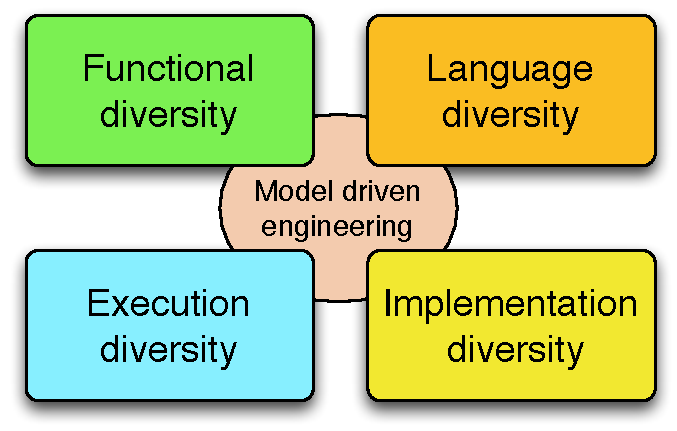
\includegraphics[width=0.5\columnwidth]{IMG/research-axis.pdf}
\caption{The four research axis of \team{}, which rely on a MDE scientific background}
\label{fig:axis}
\end{figure}

\subsection{Software Language Engineering}
\label{sec:axis-sle}

The engineering of systems involves many different stakeholders, each with their own domain of expertise. Hence more and more organizations are adopting Domain Specific Modeling Languages (DSMLs) to allow domain experts to express solutions directly in terms of relevant domain concepts   \footcite{Schmidt06,France07}. This new trend raises new challenges about designing DSMLs, evolving a set of DSMLs and coordinating the use of multiple DSLs for both DSL designers and DSL users.


\subsubsection*{Challenges} 

\textbf{Reusability} of software artifacts is a central notion that has been thoroughly studied and used by both academics and industrials since the early days of software construction. Essentially, designing reusable artifacts allows the construction of large systems from smaller parts that have been separately developed and validated, thus reducing the development costs by capitalizing on previous engineering efforts.
%
However, it is still hardly possible for language designers to design typical language artifacts (e.g. language constructs, grammars, editors or compilers) in a reusable way. The current state of the practice usually prevents the reusability of language artifacts from one language to another, consequently hindering the emergence of real engineering techniques around software languages.
Conversely, concepts and mechanisms that enable artifacts reusability abound in the software engineering community. 

\textbf{Variability} in modeling languages occur in the definition of the abstract and concrete syntax as well as in the specification of the language's semantics. 
The major challenges met when addressing the need for variability are: (i)~set principles for modeling language units that support the modular specification of a modeling language; and (ii)~design mechanisms to assemble these units in a complete language, according to the set of authorized variation points for the modeling language family.


A new generation of complex software-intensive systems (for example smart health support, smart grid, building energy management, and intelligent transportation systems) presents new opportunities for leveraging modeling languages. The development of these systems requires expertise in diverse domains.
Consequently, different types of stakeholders (e.g., scientists, engineers and end-users) must work in a coordinated manner on various aspects of the system across multiple development phases. DSMLs can be used to support the work of domain experts who focus on a specific system aspect, but they can also provide the means for coordinating work across teams specializing in different aspects and across development phases. The support and integration of DSMLs leads to what we call \textbf{the globalization of modeling languages}, \textit{i.e.} the use of multiple languages for the coordinated development of diverse aspects of a system. One can make an analogy with world globalization in which relationships are established between sovereign countries to regulate interactions (e.g., travel and commerce related interactions) while preserving each country's independent existence.


\subsubsection*{Scientific objectives} 

We address reuse and variability challenges through the investigation of the time-honored concepts of substitutability, inheritance and components, evaluate their relevance for language designers and provide tools and methods for their inclusion in software language engineering.
We will develop novel techniques for the modular construction of language extensions with the support of model syntactical variability. From the semantics perspective, we investigate extension mechanisms for the specification of variability in  operational semantics, focusing on static introduction and heterogeneous models of computation. The definition of variation points for the three aspects of the language definition provides the foundations for the novel concept Language Unit (LU) as well as suitable mechanisms to compose such units.


We explore the necessary breakthrough in software languages to support modeling and simulation of heterogeneous and open systems. This work relies on the specification of executable domain specific modeling languages (DSMLs) to formalize the various concerns of a software-intensive system, and of models of computation (MoCs) to explicitly model the concurrency, time and communication of such DSMLs. We develop a framework that integrates the necessary foundations and facilities for designing and
implementing executable and concurrent domain-specific modeling languages. It also provides unique features to specify composition operators between (possibly heterogeneous) DSMLs. Such specifications are amenable to support the edition, execution, graphical animation and analysis of heterogeneous models. The objective is to provide both a significant improvement of MoCs and DSMLs design and implementation; and the simulation based validation and verification of complex systems.


We see an opportunity for the automatic diversification of programs' computation semantics, for example through the diversification of compilers or virtual machines. The main impact of this artificial diversity is to provide flexible computation and thus ease adaptation to different execution conditions. A combination of static and dynamic analysis could support the identification of what we call \emph{plastic computation zones} in the code. We identify different categories of such zones: (i)~areas in the code in which the
order of computation can vary (e.g., the order in which a block of sequential statements is executed); (ii)~areas that can be removed, keeping the essential functionality   \footcite{Sidiroglou-Douskos2011} (e.g., skip some loop iterations); (iii)~areas that can replaced by alternative code (e.g., replace a try-catch by a return statement). Once we know which zones in the code can be randomized, it is necessary to modify the model of computation to leverage the computation plasticity. This consists in introducing variation points in the interpreter
to reflect the diversity of models of computation. Then, the choice of a given variation is performed randomly at run-time.



\subsection{Variability Modeling and Engineering}
\label{sec:axis-spl}

The systematic modeling of variability in software systems has emerged as an effective approach to document and reason about software evolutions and heterogeneity (\textit{cf.} Section~\ref{sec:variability}). Variability modeling characterizes an ``envelope'' of possible software variations. The industrial use of variability models and their relation to software artifact models require a complete engineering framework, including composition, decomposition, analysis, configuration and artifact derivation, refactoring, re-engineering, extraction, and testing.  This framework can be used both to tame imposed diversity and to manage chosen diversity.  



\subsubsection*{Challenges} 

A fundamental problem is that the \textbf{number of variants} can be exponential in the number of options (features). 
Already with 300~boolean configuration options, approximately $10^{90}$ configurations exist -- more than estimated count of atoms in the universe. Domains like automotive or operating systems have to manage more than 10000 options (e.g., Linux). Practitioners face the challenge of developing billions of variants. It is easy to forget a necessary constraint, leading to the synthesis of unsafe variants, or to under-approximate the capabilities of the software platform. Scalable modelling techniques are therefore crucial to specify and reason about a very large set of variants.

Model-driven development supports two ways to deal with the increasing number of concerns in complex systems: multi-view modeling, \textit{i.e.} when modeling each concern separately, and variability modeling. However, there is little support to combine both approaches consistently. Techniques to integrate both approaches will enable the construction of a consistent set of views and variation points in each view.

The design, construction and maintenance of software families have a major impact on \textbf{software testing}. Among the existing challenges, we can cite: the selection of test cases for a specific variant; the evolution of test suites with integration of new variants; the combinatorial explosion of the number of software configurations to be tested. Novel model-based techniques for test generation and test management in a software product line context are needed to overcome state-of-the-art limits we already observed in some projects.

\subsubsection*{Scientific objectives} 


We aim at developing scalable reasoning techniques to \textbf{automatically analyze} variability models and their interactions with other views on the software intensive system (requirements, architecture, design, code). These techniques  provide two major advancements in the  state of the art: (1)~an extension of the semantics of variability models in order to enable the definition of attributes (\textit{e.g.}, cost, quality of service, effort) on features and to include these attributes in the reasoning;  (2)~an assessment of the consistent specification of variability models with respect to system views (since variability is orthogonal to system modeling, it is currently possible to specify the different models in ways that are semantically meaningless). The former aspect of analysis is tackled through  constraint solving and finite-domain constraint programming, while the latter aspect is investigated through automatic search-based and learning-based techniques for the exploration of the space of interaction between variability and view models.

%Manual elaboration of variability models (e.g., feature models) is not realistic for large projects or for legacy systems. 
We want to develop procedures to \textbf{reverse engineer} dependencies and features' sets from existing software artefacts -- be it source code, configuration files, spreadsheets (e.g., product comparison matrices) or requirements. 
We expect to scale up (e.g., for extracting a very large number of variation points) and guarantee some properties (e.g., soundness of configuration semantics, understandability of ontological semantics). 
For instance, when building complex software-intensive systems, textual requirements are captured in very large quantities of documents. In this context, adequate models to formalize the organization of requirements documents and automated techniques to support impact analysis (in case of changes in the requirements) have to be developed.

% We also aim at developing sound methods and tools to integrate variability management in model-based testing activities. In particular, we will leverage requirement models as an essential asset to establish formal relations between variation points and test models. These relations will form the basis for novel algorithms that drive  the systematic selection of test configurations that satisfy well-defined test adequacy criteria as well as the generation of test cases for a specific product in the product line.




\subsection{Heterogeneous and dynamic software architectures}
\label{sec:axis-runtime}



Flexible yet dependable systems have to cope with heterogeneous hardware execution platforms ranging from smart sensors to huge computation infrastructures and data centers. Evolutions range from a mere change in the system configuration to a major architectural redesign,  for instance to support addition of new features or a change in the platform architecture (new hardware is made available, a running system switches to low bandwidth wireless communication, a computation node battery is running low, etc).
In this context, we need to devise formalisms to reason about the impact of an evolution and about the transition from one configuration to another.
It must be noted that this axis focuses on the use of models to drive the evolution from design time to run-time. 
Models will be used to (i)~systematically define predictable configurations and variation points through which the system will evolve;
(ii)~develop behaviors necessary to handle unpredicted evolutions.
%In the coming years, we will initiate research in this axis in the following directions.

\subsubsection*{Challenges} 

The main challenge is to provide new homogeneous architectural modelling languages and efficient techniques that enable continuous software reconfiguration to react to changes. This work handles the challenges of handling the diversity of runtime infrastructures and managing the cooperation between different stakeholders. More specifically, the research developed in this axis targets the following dimensions of software diversity.

%\textbf{Imposed diversity}

Platform architectural heterogeneity induces a first dimension of imposed diversity (type diversity). Platform reconfigurations driven by changing resources define another dimension of diversity (deployment diversity). To deal with these imposed diversity problems, we will  rely on  model based runtime support for adaptation, in the spirit of the dynamic distributed component framework developed by the Triskell team. Since the runtime environment composed of distributed, resource constrained hardware nodes cannot afford the overhead of traditional runtime adaptation techniques, we investigate the design of novel solutions relying on models@runtime and on specialized tiny virtual machines to offer resource provisioning and dynamic reconfigurations. In the next two years this research will be supported by the InfraJVM project.

%\textbf{Chosen diversity}

Diversity can also be an asset to optimize software architecture. Architecture models must integrate multiple concerns in order to properly manage the deployment of software components over a physical platform. However, these concerns can contradict each other (\textit{e.g.}, accuracy and energy). In this context, we investigate automatic solutions to explore the set of possible architecture models and to establish valid trade-offs between all concerns in case of changes. 


%projects

\subsubsection*{Scientific objectives} 

 
\textbf{Automatic synthesis of optimal software architectures.} Implementing a service over a distributed platform (\textit{e.g.}, a pervasive system or a cloud platform) consists in deploying multiple software components over distributed computation nodes. We aim at designing search-based solutions to (i)~assist the software architect in establishing a good initial architecture (that balances between different factors such as cost of the nodes, latency, fault tolerance) and to automatically update the architecture when the environment or the system itself change. The choice of search-based techniques is motivated by the very large number of possible software deployment architectures that can be investigated and that all provide different trade-offs between qualitative factors. Another essential aspect that is supported by multi-objective search is to explore different architectural solutions that are not necessarily comparable. This is important when the qualitative factors are orthogonal to each other, such as security and usability for example.

\textbf{Flexible software architecture for testing and data management.} As the number of  platforms on which software runs increases and different software versions coexist, the demand for testing environments also increases. For example, to test a  software patch or upgrade, the number of testing environments  is the product of the number of running environments the  software supports and the number of coexisting versions of the  software.  
Based on our first experiment on the synthesis of cloud environment using architectural models, our objective is to define a set of domain specific languages to catch the requirement and to design cloud environments for testing and data management of future internet systems from data centers to things. These languages will be interpreted to support dynamic synthesis and reconfiguration of a testing environment.

\textbf{Runtime support for heterogeneous environments.}
Execution environments must provide a way to account or reserve resources for applications. However, current execution environments such as the Java Virtual Machine do not clearly define a notion of application: each framework has its own definition. 
For example, in OSGi, an application is a component, in JEE, an application is most of the time associated to a class loader, in the Multi-Tasking Virtual machine, an application is a process. 
The challenge consists in defining an execution environment that provides direct control over resources (CPU, Memory, Network I/O) independently from the definition of an application. 
We propose to define abstract resource containers to account and reserve resources on a distributed network of heterogeneous devices.

\subsection{Diverse implementations for resilience}
\label{sec:axis-implementation}

Open software-intensive systems have to evolve over their lifetime in response to changes in their environment. Yet, most verification techniques assume a closed environment or the ability to predict all changes. Dynamic changes and evolutions thus represent a major challenge for these techniques that aim at assessing the correctness and robustness of the system. On the one hand, \team{} will adapt V\&V techniques to handle diversity imposed by the requirements and the execution environment, on the other hand we leverage diversity to increase the robustness of software in face of unpredicted situations. More specifically, we address the following V\&V challenges.

\subsubsection*{Challenges} 

%\textbf{Imposed diversity}

One major challenge to build flexible and open yet dependable systems is that current software engineering techniques require architects to foresee all possible  situations the system will have to face. However, openness and flexibility also mean unpredictability: unpredictable bugs, attacks, environmental evolutions, etc. Current fault-tolerance   \footcite{randell75} and security   \footcite{forrest1997building} techniques  provide software systems with the capacity of detecting   accidental and deliberate faults. However, existing solutions assume that the set of bugs or vulnerabilities in a system does not evolve. This assumption does not hold for open systems, thus it is essential to revisit fault-tolerance and security solutions to account for diverse and unpredictable faults.

%\textbf{Chosen diversity}

Diversity is known to be a major asset for the robustness of large, open, and complex systems (\textit{e.g.}, economical or ecological systems). 
Following this observation, the software engineering literature provides a rich set of work that choose to implement diversity in software systems in order to improve robustness to attacks or to changes in quality of service. 
These works range from N-version programming to obfuscation of data structures or control flow, to randomization of instruction sets. 
An essential remaining challenge is to support the automatic synthesis and evolution of software diversity in open software-intensive systems.
There is an opportunity to further enhance these techniques in order to cope with a wider diversity of faults, by multiplying the levels of diversity in the different software layers that are found in software-intensive systems (system, libraries, frameworks, application). 
This increased diversity must be based on artificial program transformations and code synthesis, which increase the chances of exploring novel solutions, better fitted at one point in time. The biological analogy also indicates that diversity should emerge as a side-effect of evolution, to prevent over-specialization towards one kind of diversity.


\subsubsection*{Scientific objectives} 

The main objective is to address one of the main limitations of N-version programming for fault-tolerant systems: the manual production and management of software diversity. Through automated injection of artificial diversity we aim at systematically increasing failure diversity and thus increasing the chances of early error detection at run-time. A fundamental assumption for this work is that software-intensive systems can be ``good enough''   \footcite{Rinard12, Zhu12}. 

\textbf{Proactive program diversification.} We aim at establishing novel principles and techniques that favor the emergence of multiple forms of software diversity in software-intensive systems, in conjunction with the software adaptation mechanisms that leverage this diversity. The main expected outcome is a set of meta-design principles that maintain diversity in systems and the experimental demonstration of the effects of software diversity on the
adaptive capacities of CASs. Higher levels of diversity in the system provide a pool of software solutions that can eventually be used to adapt to  situations unforeseen at design time (bugs, crash, attacks, etc.). Principles of automated software diversification rely on the automated synthesis of variants in a software product line, as well as finer-grained program synthesis combining unsound transformations and genetic programming to explore the space of mutational robustness.

\textbf{Multi-tier software diversification.} We call  multi-tier diversification the fact of diversifying several application software components simultaneously. The novelty of our proposal, with respect to the software diversity state of the art, is to diversify the application-level code (for example, diversify the business logics of the application), focusing on the technical layers found in web applications. 
The diversification of application software code is expected to provide a diversity of failures and vulnerabilities in web server deployment. 
Web server deployment usually adopts a form of the Reactor architecture pattern, for scalability purposes: multiple copies of the server software stack, called request handlers, are deployed behind a load balancer. 
This architecture is very favorable for diversification, since by using the multiplicity of request handlers running in a web server we can simultaneously deploy multiple combinations of diverse software components. Then, if one handler is hacked or crashes the others should still be able to process client requests.


\end{module}







%%%%%%%%%%%%%%%%%%%%%%%%%%%%%%%%%%%%%%%%%%%%%%%%%%%%%%%%%%%%%%%%%%%%%%%%%%%
%%%
%%% Section Highlights (Faits Marquants)
%%%  
%%% Les faits marquants doivent être relatifs aux résultats de l'année obtenus par votre équipe.
%%% L'obtention d'une HDR n'est pas un fait marquant.
%%% La sous-partie Awards (précédemment "Best papers") vous permet de signaler toute récompense, concernant une publication ou pas.  
%%% Tous types de publication récompensée peuvent être présentés ici. La récompense doit dater de l'année, la publication pas forcément.
%%% Citez-les dans la partie "Awards" sous la forme : \bestcite{xxxx}, \bestcite{yyyy}, ...  
%%%
%%% Documentation intranet : https://intranet.inria.fr/Vie-scientifique/Information-edition-scientifiques/RAweb/Les-sections#eztoc27554_8
%%%  
%%%
%%%%%%%%%%%%%%%%%%%%%%%%%%%%%%%%%%%%%%%%%%%%%%%%%%%%%%%%%%%%%%%%%%%%%%%%%%%%

\begin{module}{highlights}{NewHighlights}{}


JHipster article at ESEM~\cite{halin:hal-01829928}

\subsection{Awards}

%% ICI vous pouvez ecrire du texte
%%
%% citez les "Awards" sous la forme : \bestcite{xxxx}, \bestcite{yyyy}, ...

\end{module}

%%%%%%%%%%%%%%%%%%%%%%%%%%%%%%%%%%%%%%%%%%%%%%%%%%%%%%%%%%%%%%%%%%%%%%%%%%%%%%
%%%
%%% Section logiciels et plateformes
%%%
%%%
%%% Information sur les données importées : logiciels
%%%  
%%% Il n'est pas possible de modifier le tex de la partie logiciel de cette section : les logiciels sont importés de la base BIL.  
%%% Il faut passer par BIL (https://bil.inria.fr/fr/catalog/listby/raweb) pour rajouter et compléter des logiciels.  
%%% Critères de sélection des logiciels pour le RA : avoir été développé ou avoir connu une évolution majeure ou importante en 2018.
%%% Le fichier tex du rapport est mis à jour automatiquement à chaque compilation.
%%% Il faut ensuite consulter le rapport en HTML et/ou en PDF pour vérifier le résultat.
%%%  
%%% Par contre la partie pour les platformes doit toujours être mise à jour manuellement à partir de ce fichier tex.
%%%
%%% Documentation intranet : https://intranet.inria.fr/Vie-scientifique/Information-edition-scientifiques/RAweb/Les-sections#eztoc27554_9
%%%
%%% En cas de problème : https://helpdesk.inria.fr/categories/181/submit
%%%
%%%%%%%%%%%%%%%%%%%%%%%%%%%%%%%%%%%%%%%%%%%%%%%%%%%%%%%%%%%%%%%%%%%%%%

%%%
%%% Ici la section logiciel va être incluse à la compilation    
%%% Il est possible de consulter le source tex qui va être inclus à l'adresse suivante :  
%%%     https://irabot.inria.fr/itramera?format=bil&epi=diverse&annee=2018
%%%
%%%
%%% La partie Plaforms de la section logiciels et plateformes doit, le cas échéant, être complétée ici :  
%%%  

 \begin{module}{logiciels}{bil-2737}{amiunique}

   \textsc{Keywords:} Privacy - Browser fingerprinting \\ 


    \textsc{Scientific Description:} The amiunique web site has been deployed in the context of the DiverSE's research activities on browser fingerprinting and how software diversity can be leveraged in order to mitigate the impact of fingerprinting on the privacy of users. The construction of a dataset of genuine fingerprints is essential to understand in details how browser fingerprints can serve as unique identifiers and hence what should be modified in order to mitigate its impact privacy. This dataset also supports the large-scale investigation of the impact of web technology advances on fingerprinting. For example, we can analyze in details the impact of the HTML5 canvas element or the behavior of fingerprinting on mobile devices.

The whole source code of amiunique is open source and is distributed under the terms of the MIT license.

Similar sites:
    Panopticlick https://panopticlick.eff.org/
    BrowserSpy http://browserspy.dk/
    http://noc.to/
Main innovative features:
    canvas fingerprinting
    WebGL fingerprinting
    advanced JS features (platform, DNT, etc.)

Impact:
The website has been showcased in several professional forums in 2014 and 2015 (Open World Forum 2014, FOSSA'14, FIC'15, ICT'15) and it has been visited by more than 100000 unique visitors in one year.\\

 \textsc{Functional Description:}  This web site aims at informing visitors about browser fingerprinting and possible tools to mitigate its effect, as well as at collecting data about the fingerprints that can be found on the web. It collects browser fingerprints with the explicit agreement of the users (they have to click on a button on the home page). Fingerprints are composed of 17 attributes, which include regular HTTP headers as well as the most recent state of the art techniques (canvas fingerprinting, WebGL information).\\

   \begin{itemize}
      \item Participants: Benoit Baudry and Pierre Laperdrix
      \item Partner: INSA Rennes
          % Contact: Vérifiez si cette personne est toujours membre de Inria.
    % Sinon corrigez la BIL (base des logiciels Inria): https://bil.inria.fr/ 
      \item Contact: Benoit Baudry
      \item URL: \url{https://amiunique.org/}
   \end{itemize}

 \end{module}

 \begin{module}{logiciels}{bil-1468}{FAMILIAR}

   \textsc{Keywords:} Software line product - Configators - Customisation \\ 


    \textsc{Scientific Description:} FAMILIAR (for FeAture Model scrIpt Language for manIpulation and Automatic Reasoning) is a language for importing, exporting, composing, decomposing, editing, configuring, computing "diffs", refactoring, reverse engineering, testing, and reasoning about (multiple) feature models. All these operations can be combined to realize complex variability management tasks. 
A comprehensive environment is proposed as well as integration facilities with the Java ecosystem.\\

 \textsc{Functional Description:}  Familiar is an environment for large-scale product customisation. From a model of product features (options, parameters, etc.), Familiar can automatically generate several million variants. These variants can take many forms: software, a graphical interface, a video sequence or even a manufactured product (3D printing). Familiar is particularly well suited for developing web configurators (for ordering customised products online), for providing online comparison tools and also for engineering any family of embedded or software-based products.\\

   \begin{itemize}
    %  \item Participants: Mathieu Acher, Hugo Martin, Olivier Barais
          % Contact: Vérifiez si cette personne est toujours membre de Inria.
    % Sinon corrigez la BIL (base des logiciels Inria): https://bil.inria.fr/ 
      \item Contact: Mathieu Acher
      \item URL: \url{http://familiar-project.github.com}
   \end{itemize}

 \end{module}

 \begin{module}{logiciels}{bil-2742}{GEMOC Studio}

   \textsc{Keywords:} DSL - Language workbench - Model debugging \\ 


    \textsc{Scientific Description:} The language workbench put together the following tools seamlessly integrated to the Eclipse Modeling Framework (EMF):

- Melange, a tool-supported meta-language to modularly define executable modeling languages with execution functions and data, and to extend (EMF-based) existing modeling languages.
- MoCCML, a tool-supported meta-language dedicated to the specification of a Model of Concurrency and Communication (MoCC) and its mapping to a specific abstract syntax and associated execution functions of a modeling language.
- GEL, a tool-supported meta-language dedicated to the specification of the protocol between the execution functions and the MoCC to support the feedback of the data as well as the callback of other expected execution functions.
- BCOoL, a tool-supported meta-language dedicated to the specification of language coordination patterns to automatically coordinates the execution of, possibly heterogeneous, models.
- Sirius Animator, an extension to the model editor designer Sirius to create graphical animators for executable modeling languages.\\

 \textsc{Functional Description:}  The GEMOC Studio is an eclipse package that contains components supporting the GEMOC methodology for building and composing executable Domain-Specific Modeling Languages (DSMLs). It includes the two workbenches:
    The GEMOC Language Workbench: intended to be used by language designers (aka domain experts), it allows to build and compose new executable DSMLs.
    The GEMOC Modeling Workbench: intended to be used by domain designersto create, execute and coordinate models conforming to executable DSMLs. The different concerns of a DSML, as defined with the tools of the language workbench, are automatically deployed into the modeling workbench. They parametrize a generic execution framework that provide various generic services such as graphical animation, debugging tools, trace and event managers, timeline, etc.\\

   \begin{itemize}
      \item Participants: Didier Vojtisek, Dorian Leroy, Erwan Bousse, Fabien Coulon and Julien Deantoni
      \item Partners: IRIT - ENSTA - I3S - OBEO - Thales TRT
          % Contact: Vérifiez si cette personne est toujours membre de Inria.
    % Sinon corrigez la BIL (base des logiciels Inria): https://bil.inria.fr/ 
      \item Contact: Benoît Combemale
      \item URL: \url{http://gemoc.org/studio.html}
   \end{itemize}

 \end{module}

 \begin{module}{logiciels}{bil-376}{Kevoree}

 \textit{Kevoree Core} \\ 


   \textsc{Keywords:} M2M - Dynamic components - Iot - Heterogeneity - Smart home - Cloud - Software architecture - Dynamic deployment \\ 


    \textsc{Scientific Description:} Kevoree is an open-source models@runtime platform (http://www.kevoree.org) to properly support the dynamic adaptation of distributed systems. Models@runtime basically pushes the idea of reflection one step further by considering the reflection layer as a real model that can be uncoupled from the running architecture (e.g. for reasoning, validation, and simulation purposes) and later automatically resynchronized with its running instance.

Kevoree has been influenced by previous work that we carried out in the DiVA project and the Entimid project. With Kevoree we push our vision of models@runtime farther. In particular, Kevoree provides a proper support for distributed models@runtime. To this aim we introduced the Node concept to model the infrastructure topology and the Group concept to model semantics of inter node communication during synchronization of the reflection model among nodes. Kevoree includes a Channel concept to allow for multiple communication semantics between remoteComponents deployed on heterogeneous nodes. All Kevoree concepts (Component, Channel, Node, Group) obey the object type design pattern to separate deployment artifacts from running artifacts. Kevoree supports multiple kinds of very different execution node technology (e.g. Java, Android, MiniCloud, FreeBSD, Arduino, ...).

Kevoree is distributed under the terms of the LGPL open source license.

\textsc{Main competitors:}
\begin{itemize}
	\item the Fractal/Frascati eco-system (http://frascati.ow2.org ).
 	\item SpringSource Dynamic Module (http://spring.io/ )
 	\item GCM-Proactive (http://proactive.inria.fr/ )
 	\item OSGi (http://www.osgi.org ) 
 	\item Chef
 	\item Vagran (http://vagrantup.com/ )
\end{itemize}
    GCM-Proactive (http://proactive.inria.fr/ )

    OSGi (http://www.osgi.org )

\textsc{Main innovative features:}
\begin{itemize}
	\item distributed models@runtime platform (with a distributed reflection model and an extensible models@runtime dissemination set of strategies).
	\item Support for heterogeneous node type (from Cyber Physical System with few resources until cloud computing infrastructure).
	\item Fully automated provisioning model to correctly deploy software modules and their dependencies.
	\item Communication and concurrency access between software modules expressed at the model level (not in the module implementation).
\end{itemize}

    Vagran (http://vagrantup.com/ )

\textsc{Impact:} Several tutorials and courses have been performed this year at EJCP for French PhD student, at ECNU summer school for 82 chineese PhD students. See also the web page http://www.kevoree.org .

In 2015, we mainly created a new implementation in C\# and we created an implementation for system containers for driving resources using Kevoree. We also use Kevoree in the context of Mohammed's PhD to create testing infrastructure on-demand.\\

 \textsc{Functional Description:}  Kevoree is an open-source models@runtime platform to properly support the dynamic adaptation of distributed systems. Models@runtime basically pushes the idea of reflection one step further by considering the reflection layer as a real model that can be uncoupled from the running architecture (e.g. for reasoning, validation, and simulation purposes) and later automatically resynchronized with its running instance.\\

   \begin{itemize}
      \item Participants: Aymeric Hervieu, Benoit Baudry, Francisco-Javier Acosta Padilla, Inti Gonzalez Herrera, Ivan Paez Anaya, Jacky Bourgeois, Jean Emile Dartois, Johann Bourcier, Manuel Leduc, Maxime Tricoire, Mohamed Boussaa, Noël Plouzeau and Olivier Barais
          % Contact: Vérifiez si cette personne est toujours membre de Inria.
    % Sinon corrigez la BIL (base des logiciels Inria): https://bil.inria.fr/ 
      \item Contact: Olivier Barais
      \item URL: \url{http://kevoree.org/}
   \end{itemize}

 \end{module}

 \begin{module}{logiciels}{bil-2731}{Melange}

   \textsc{Keywords:} Model-driven engineering - Meta model - MDE - DSL - Model-driven software engineering - Dedicated langage - Language workbench - Meta-modelisation - Modeling language - Meta-modeling \\ 


    \textsc{Scientific Description:} Melange is a follow-up of the executable metamodeling language Kermeta, which provides a tool-supported dedicated meta-language to safely assemble language modules, customize them and produce new DSMLs. Melange provides specific constructs to assemble together various abstract syntax and operational semantics artifacts into a DSML. DSMLs can then be used as first class entities to be reused, extended, restricted or adapted into other DSMLs. Melange relies on a particular model-oriented type system that provides model polymorphism and language substitutability, i.e. the possibility to manipulate a model through different interfaces and to define generic transformations that can be invoked on models written using different DSLs. Newly produced DSMLs are correct by construction, ready for production (i.e., the result can be deployed and used as-is), and reusable in a new assembly.

Melange is tightly integrated with the Eclipse Modeling Framework ecosystem and relies on the meta-language Ecore for the definition of the abstract syntax of DSLs. Executable meta-modeling is supported by weaving operational semantics defined with Xtend. Designers can thus easily design an interpreter for their DSL in a non-intrusive way. Melange is bundled as a set of Eclipse plug-ins.\\

 \textsc{Functional Description:}  Melange is a language workbench which helps language engineers to mashup their various language concerns as language design choices, to manage their variability, and support their reuse. It provides a modular and reusable approach for customizing, assembling and integrating DSMLs specifications and implementations.\\

   \begin{itemize}
      \item Participants: Arnaud Blouin, Benoît Combemale, David Mendez Acuna, Didier Vojtisek, Dorian Leroy, Erwan Bousse, Fabien Coulon, Jean-Marc Jézéquel, Olivier Barais and Thomas Degueule
          % Contact: Vérifiez si cette personne est toujours membre de Inria.
    % Sinon corrigez la BIL (base des logiciels Inria): https://bil.inria.fr/ 
      \item Contact: Benoît Combemale
      \item URL: \url{http://melange-lang.org}
   \end{itemize}

 \end{module}

 \begin{module}{logiciels}{bil-2580}{Opencompare}

   \textsc{Keyword:} Software Product Line \\ 


   

 \textsc{Functional Description:}  Product comparison matrices (PCMs) are tabular data: supported and unsupported features are documented for both describing the product itself and for discriminating one product compared to another. PCMs abound – we are all using PCMs – and constitute a rich source of knowledge for easily comparing and choosing product. Yet the current practice is suboptimal both for humans and computers, mainly due to unclear semantics, heterogeneous forms of data, and lack of dedicated support. 

OpenCompare.org is an ambitious project for the collaborative edition, the sharing, the standardisation, and the open exploitation of PCMs. The goal of OpenCompare.org is to provide an integrated set of tools (e.g., APIs, visualizations, configurators, editors) for democratizing their creation, import, maintenance, and exploitation.\\

   \begin{itemize}
      \item Participants: Guillaume Bécan, Mathieu Acher and Sana Ben Nasr
          % Contact: Vérifiez si cette personne est toujours membre de Inria.
    % Sinon corrigez la BIL (base des logiciels Inria): https://bil.inria.fr/ 
      \item Contact: Mathieu Acher
      \item URL: \url{http://opencompare.org}
   \end{itemize}

 \end{module}

 \begin{module}{logiciels}{bil-2938}{DSpot}

   \textsc{Keywords:} Software testing - Test amplification \\ 


   

 \textsc{Functional Description:}  DSpot is a tool that generates missing assertions in JUnit tests. DSpot takes as input a Java project with an existing test suite. As output, DSpot outputs new test cases on console. DSpot supports Java projects built with Maven and Gradle\\

   \begin{itemize}
      \item Participants: Benoit Baudry, Martin Monperrus and Benjamin Danglot
      \item Partner: KTH Royal Institute of Technology
          % Contact: Vérifiez si cette personne est toujours membre de Inria.
    % Sinon corrigez la BIL (base des logiciels Inria): https://bil.inria.fr/ 
      \item Contact: Benjamin Danglot
      \item URL: \url{https://github.com/STAMP-project/dspot}
   \end{itemize}

 \end{module}

 \begin{module}{logiciels}{bil-3337}{ALE}

 \textit{Action Language for Ecore} \\ 


   \textsc{Keywords:} Meta-modeling - Executable DSML \\ 


   

 \textsc{Functional Description:}  Main features of ALE include:

\begin{itemize}
	\item Executable metamodeling: Re-open existing EClasses to insert new methods with their implementations
	\item Metamodel extension: The very same mechanism can be used to extend existing Ecore metamodels and insert new features (eg. attributes) in a non-intrusive way
	\item Interpreted: No need to deploy Eclipse plugins, just run the behavior on a model directly in your modeling environment
	\item Extensible: If ALE doesn’t fit your needs, register Java classes as services and invoke them inside your implementations of EOperations.
\end{itemize}


   \begin{itemize}
      \item Partner: OBEO
          % Contact: Vérifiez si cette personne est toujours membre de Inria.
    % Sinon corrigez la BIL (base des logiciels Inria): https://bil.inria.fr/ 
      \item Contact: Benoît Combemale
      \item URL: \url{http://gemoc.org/ale-lang/}
   \end{itemize}

 \end{module}

  \begin{module}{logiciels}{bil-3338}{Descartes}
	
	\textsc{Keywords:} Mutation testing - Mutation analysis - Java - JUnit - PIT \\ 
	
	
	
	
	\textsc{Functional Description:}  Descartes evaluates the capability of your test suite to detect bugs using extreme mutation testing. In Extreme Mutation testing, the whole body of a method under test is removed. Descartes is a mutation engine plugin for PIT which implements extreme mutation operators. It provides reports combining, line coverage, mutation score and list of weaknesses in the source.\\
	
	\begin{itemize}
		\item Participants: Benoit Baudry, Caroline Landry, Oscar luis Vera-Perez
		% Contact: Vérifiez si cette personne est toujours membre de Inria.
		% Sinon corrigez la BIL (base des logiciels Inria): https://bil.inria.fr/ 
		\item Contact: Oscar luis Vera-Perez
		\item Partner: ATOS, CSQE, Engineering, INRIA, KTH, XWiki
		\item URL: \url{https://github.com/STAMP-project/pitest-descartes\begin{center}
				https://github.com/STAMP-project/pitest-descartes
		\end{center}}
	\end{itemize}
\end{module}

\begin{module}{logiciels}{bil-3448}{PitMP}
	
	\textsc{Keywords:} Mutation testing - Mutation analysis - Java - JUnit - PIT - Maven - Multi-module project \\ 
	
	\textsc{Functional Description:}  PitMP (PIT for Multi-module Project) is a Maven plugin able to run PIT and Descartes on multi-module projects. PIT is a mutation testing system for Java applications, which allows you to evaluate the quality of your test suites.\\
	
	\begin{itemize}
		\item Participants: Benoit Baudry, Caroline Landry, Oscar luis Vera-Perez
		% Contact: Vérifiez si cette personne est toujours membre de Inria.
		% Sinon corrigez la BIL (base des logiciels Inria): https://bil.inria.fr/ 
		\item Contact: Caroline Landry
		\item Partner: CSQE, Engineering, INRIA, KTH, XWiki
		\item URL: \url{https://github.com/STAMP-project/pitmp-maven-plugin\begin{center}
				https://github.com/STAMP-project/pitmp-maven-plugin
		\end{center}}
	\end{itemize}
	
\end{module}


\begin{module}{logiciels}{bil-3339}{InspectorGuidget}

   \textsc{Keywords:} Static analysis - Software testing - User Interfaces \\ 


   

 \textsc{Functional Description:}  InspectorGuidget is a static code analysing tool. InspectorGuidget analyses UI (user interface/interaction) code  of a software system to extract high level information and metrics. InspectorGuidget also finds bad UI coding pratices, such as Blob listener instances. InspectorGuidget analyses Java code.\\

   \begin{itemize}
      \item Participants: Arnaud Blouin and Benoit Baudry
      \item Status: prototype, applied on large scale applications
      \item Size: 1k Java LoC
          % Contact: Vérifiez si cette personne est toujours membre de Inria.
    % Sinon corrigez la BIL (base des logiciels Inria): https://bil.inria.fr/ 
      \item Contact: Arnaud Blouin
      \item Publications: \href{https://hal.inria.fr/hal-01499106v5}{hal-01499106v5} - 
 \href{https://hal.inria.fr/hal-01308625v2}{hal-01308625v2}
      \item URL: \url{https://github.com/diverse-project/InspectorGuidget}
   \end{itemize}

 \end{module}



%%%%%%%%%%%%%%%%%%%%%%%%%%%%%%%%%%%%%%%%%%%%%%%%%%%%%%%
%%%
%%% Section Resultat nouveaux (New Results)
%%% Il y a des modules ici

%%%Documentation intranet : https://intranet.inria.fr/Vie-scientifique/Information-edition-scientifiques/RAweb/Les-sections#eztoc27554_10
%%%%%%%%%%%%%%%%%%%%%%%%%%%%%%%%%%%%%%%%%%%%%%%%%%%%%%%%

\begin{module}{resultats}{results-spl}{Results on Variability modeling and management}
	\label{sec:results-spl}
	% We select three main contributions for this DiverSE's research axis.
% Two contributions are in the field of variability model synthesis, while the third one is in the field of variability testing.



    
    
    
	% We hope to gather more and more data (open data like Wikipedia) and offer innovative services on top of our canonical format.
	% Papers have been notably published at FSE'13, ASE'13 and ASE'14 (ASE and FSE are leading conferences in software engineering), SPLC'15 (SPLC is a leading conference in variability). %%% TODO JSS.
%	\end{description}


% \end{description}

\paragraph{Variability and testing.}
Many approaches for testing configurable software systems start from the same assumption: it is impossible to test all configurations. This motivated the definition of variability-aware abstractions and sampling techniques to cope with large configuration spaces. Yet, there is no theoretical barrier that prevents the exhaustive testing of all configurations by simply enumerating them, if the effort required to do so remains acceptable. Not only this: we believe there is lots to be learned by systematically and exhaustively testing a configurable system. We report on the first ever endeavor to test all possible configurations of an industry-strength, open source configurable software system, JHipster, a popular code generator for web applications. We built a testing scaffold for the 26,000+ configurations of JHipster using a cluster of 80 machines during 4 nights for a total of 4,376 hours (182 days) CPU time. We find that 35.70\% configurations fail and we identify the feature interactions that cause the errors. We show that sampling testing strategies (like dissimilarity and 2-wise) (1) are more effective to find faults than the 12 default configurations used in the JHipster continuous integration; (2) can be too costly and exceed the available testing budget. We cross this quantitative analysis with the qualitative assessment of JHipster's lead developers.
Publication at Empirical Software Engineering: ~\cite{halin:hal-01829928}
See also, in the rest of the report, the work on \emph{Multimorphic Testing} that actually relies on variability techniques. 
% preliminary effort on JHipster~\cite{halin:hal-01468084}, \url{https://arxiv.org/abs/1710.07980} \url{https://github.com/axel-halin/Thesis-JHipster/}


\paragraph{Variability and teaching.}

Software Product Line (SPL) engineering has emerged to provide the means to efficiently model, produce, and maintain multiple similar software variants, exploiting their common properties, and managing their variabilities (differences). With over two decades of existence, the community of SPL researchers and practitioners is thriving as can be attested by the extensive research output and the numerous successful industrial projects. Education has a key role to support the next generation of practitioners to build highly complex, variability-intensive systems. Yet, it is unclear how the concepts of variability and SPLs are taught, what are the possible missing gaps and difficulties faced, what are the benefits, or what is the material available. Also, it remains unclear whether scholars teach what is actually needed by industry. We report on three initiatives we have conducted with scholars, educators, industry practitioners, and students to further understand the connection between SPLs and education, i.e., an online survey on teaching SPLs we performed with 35 scholars, another survey on learning SPLs we conducted with 25 students, as well as two workshops held at the International Software Product Line Conference in 2014 and 2015 with both researchers and industry practitioners participating. We build upon the two surveys and the workshops to derive recommendations for educators to continue improving the state of practice of teaching SPLs, aimed at both individual educators as well as the wider community. Finally, we are developing and maintaining a repository for teaching SPLs and variability.
Publication at SPLC (journal first)~\cite{acher:hal-01829933}, workshop SPLTea'18 \url{http://spltea.irisa.fr/} and repository: \url{https://teaching.variability.io}

%\paragraph{Variability and constraint solving.}  
%Array constraints are essential for handling data structures in automated reasoning and software verification. Unfortunately, the use of a typical finite domain (FD) solver based on local consistency-based filtering has strong limitations when constraints on indexes are combined with constraints on array elements and size. This work proposes an efficient and complete FD-solving technique for extended constraints over (possibly unbounded) arrays. We describe a simple but particularly powerful transformation for building an equisatisfiable formula that can be efficiently solved using standard FD reasoning over arrays, even in the unbounded case. Experiments show that the proposed solver significantly outperforms FD solvers, and successfully competes with the best SMT-solvers~\cite{plazar:hal-01545557}.
% This work is not directly related to variability and SPL. 
% But it contributes to DiverSE's attempts to connect artificial intelligence techniques to software variability engineering, in which constraint solving or machine learning are typically applied. 

\paragraph{Variability and machine learning}
%\begin{description}
%	\item[Contribution.] 
We propose the use of a machine learning approach to infer variability constraints
from an oracle that is able to assess whether a given configuration is correct.
We propose an automated procedure to generate configurations, classify them according to the oracle, and synthesize cross-tree constraints. Specifically, based on an oracle (e.g. a runtime test) that tells us whether a given configuration meets the requirements (e.g. speed or memory footprint), we leverage machine learning to retrofit the acquired knowledge into a variability model of the system that can be used to automatically specialize the configurable system. We validate our approach on a set of well-known configurable software systems (Apache server, x264, etc.) 
Our results show that, for many different kinds of objectives and performance qualities, the approach has interesting accuracy, precision and recall after a learning stage based on a relative small number of random samples.
Publications: Temple et al. \emph{Towards Adversarial Configurations for Software Product Lines} \url{https://arxiv.org/abs/1805.12021}, VaryLaTeX~\cite{acher:hal-01659161} a variability and learning-based tool to generate relevant paper variants written in \latex. 

\emph{TUXML (Tux is the mascotte of the Linux Kernel while ML stands for statistical machine learning)}. The goal of TuxML  is to predict properties of Linux Kernel configurations (e.g., does the kernel compile? what's its size? does it boot?). The Linux Kernel provides near 15000 configuration options: there is an infinity of different kernels. As we cannot compile, measure, and observe all combinations of options (aka configurations), we're trying to learn Linux kernel properties out of a sample of configurations. The TuxML project is developing tools, mainly based on Docker and Python, to massively compile and gather data about thousand of configuration kernels~\url{https://github.com/TuxML/}.

In general, we are currently exploring the use of machine learning for variability-intensive systems in the context of VaryVary ANR project \url{https://varyvary.github.io}.




%\subsection{Reverse engineering variability}
%
%We have developed automated techniques and a comprehensive environment for synthesizing feature models from various kinds of artefacts (e.g. propositional formula, dependency graph, FMs or product comparison matrices). Specifically we have elaborated a support (through ranking lists, clusters, and logical heuristics) for choosing a sound and meaningful hierarchy. 
%We have performed an empirical evaluation on hundreds of feature models, coming from the SPLOT repository and Wikipedia.
%% We have provided evidence that a fully automated synthesis (i.e., without any user intervention) is likely to produce models far from the ground truths. 
%We have showed that a hybrid approach mixing logical and ontological techniques
%outperforms state-of-the-art solutions (Empirical Software Engineering journal in 2016~\cite{becan:hal-01096969}). 
%
%
%% We have also considered numerical information and feature \emph{attributes} so that we are now capable of synthesizing attributed feature models from product descriptions~\cite{becan:hal-01178454}. 
%
%% Besides, we have developed techniques for reverse engineering variability in generators and configurators (e.g., video generators)~\cite{becan:hal-01104797}. 
%% We have identified new research directions for protecting variability~\cite{acher:hal-01234342} mainly due to the fact reverse engineering techniques (previously presented) are effective .
%
%
%\subsection{Product comparison matrices}
%
%Product Comparison Matrices (PCMs) constitute a rich source of data for comparing a set of related and competing products over numerous features. PCMs can be seen as a formalism for modeling a family of products, including variability information.
%Despite their apparent simplicity, PCMs contain heterogeneous, ambiguous, uncontrolled and partial information that hinders their efficient exploitations. 
%We have formalized PCMs through model-based automated techniques and developed additional tooling to support the edition and re-engineering of PCMs~\cite{becan:hal-01058440}. 20 participants used our editor to evaluate our PCM metamodel and automated transformations. The empirical results over 75 PCMs from Wikipedia show that (1) a significant proportion of the formalization of PCMs can be automated: 93.11\% of the 30061 cells are correctly formalized; (2) the rest of the formalization can be realized by using the editor and mapping cells to existing concepts of the metamodel. 
%%
% % The ASE'2014 paper opens avenues for engaging a community in the mining, re-engineering, edition, and exploitation of PCMs that now abound on the Internet.
%We have launched an open, collaborative initiative towards this direction \url{http://www.opencompare.org}
%
%Another axis is the mining of PCMs since (1) the manual elaboration of PCMs has limitations (2) numerous sources of information can be combined and are amenable to PCMs. We have developed MatrixMiner a tool for automatically
%synthesizing PCMs from a set of product descriptions written in natural language~\cite{JSSbennasr}. %%% TODO JSS
%MatrixMiner is capable of identifying and organizing
%features and values in a PCM despite the informality and
%absence of structure in the textual descriptions of products. 
%More information is available online: \url{http://matrix-miner.variability.io}
\end{module}

\begin{module}{resultats}{results-implem-sle}{Results on Software Language
		Engineering}
	\label{sec:results-sle}
	\paragraph{Omniscient Debugging for Executable DSLs}

Omniscient debugging is a promising technique that relies on execution traces to enable free traversal of the states reached by a model (or program) during an execution. While a few General-Purpose Languages (GPLs) already have support for omniscient debugging, developing such a complex tool for any executable Domain Specific Language (DSL) remains a challenging and error prone task. A generic solution must: support a wide range of executable DSLs independently of the metaprogramming approaches used for implementing their semantics; be efficient for good responsiveness. Our contribution in \cite{bousse:hal-01662336} relies on a generic omniscient debugger supported by efficient generic trace management facilities. To support a wide range of executable DSLs, the debugger provides a common set of debugging facilities, and is based on a pattern to define runtime services independently of metaprogramming approaches. Results show that our debugger can be used with various executable DSLs implemented with different metaprogramming approaches. As compared to a solution that copies the model at each step, it is on average six times more efficient in memory, and at least 2.2 faster when exploring past execution states, while only slowing down the execution 1.6 times on average.

\paragraph{Trace Comprehension Operators for Executable DSLs}

Recent approaches contribute facilities to breathe life into metamodels, thus making behavioral models directly executable. Such facilities are particularly helpful to better utilize a model over the time dimension, e.g., for early validation and verification. However, when even a small change is made to the model, to the language definition (e.g., semantic variation points), or to the external stimuli of an execution scenario, it remains difficult for a designer to grasp the impact of such a change on the resulting execution trace. This prevents accessible trade-off analysis and design-space exploration on behavioral models. In \cite{leroy:hal-01803031}, we propose a set of formally defined operators for analyzing execution traces. The operators include dynamic trace filtering, trace comparison with diff computation and visualization, and graph-based view extraction to analyze cycles. The operators are applied and validated on a demonstrative example that highlight their usefulness for the comprehension specific aspects of the underlying traces.

\paragraph{Model Transformation Reuse across Metamodels}
Model transformations (MTs) are essential elements of model-driven engineering (MDE) solutions. MDE promotes the creation of domain-specific metamodels, but without proper reuse mechanisms, MTs need to be developed from scratch for each new metamodel. In \cite{bruel:hal-01910113}, awarded by the \textbf{best paper award at ICMT 2018}, we classify reuse approaches for MTs across different metamodels and compare a sample of specific approaches -- model types, concepts, a-posteriori typing, multilevel modeling, and design patterns for MTs -- with the help of a feature model developed for this purpose, as well as a common example. We discuss strengths and weaknesses of each approach, provide a reading grid used to compare their features, and identify gaps in current reuse approaches.

\paragraph{Modular Language Composition for the Masses}
The goal of modular language development is to enable the definition of new languages as assemblies of pre-existing ones. Recent approaches in this area are plentiful but usually suffer from two main problems: either they do not support modular language composition both at the specification and implementation levels, or they require advanced knowledge of specific paradigms which hampers wide adoption in the industry. In \cite{leduc:hal-01890446}, awarded by the \textbf{best artefact award at SLE 2018}, we introduce a non-intrusive approach to modular development of language concerns with well-defined interfaces that can be composed modularly at the specification and implementation levels. We present an implementation of our approach atop the Eclipse Modeling Framework, namely Alex-an object-oriented metalanguage for semantics definition and language composition. We evaluate Alex in the development of a new DSL for IoT systems modeling resulting from the composition of three independently defined languages (UML activity diagrams, Lua, and the OMG Interface Description Language). We evaluate the effort required to implement and compose these languages using Alex with regards to similar approaches of the literature.

\paragraph{Shape-Diverse DSLs}
Domain-Specific Languages (DSLs) manifest themselves in remarkably diverse shapes, ranging from internal DSLs embedded as a mere fluent API within a programming language, to external DSLs with dedicated syntax and tool support. Although different shapes have different pros and cons, combining them for a single language is problematic: language designers usually commit to a particular shape early in the design process, and it is hard to reconsider this choice later. In the new ideas paper \cite{coulon:hal-01889155} awarded as the \textbf{best new ideas paper at SLE 2018}, we envision a language engineering approach enabling (i) language users to manipulate language constructs in the most appropriate shape according to the task at hand, and (ii) language designers to combine the strengths of different technologies for a single DSL. We report on early experiments and lessons learned building Prism, our prototype approach to this problem. We illustrate its applicability in the engineering of a simple shape-diverse DSL implemented conjointly in Rascal, EMF, and Java. We hope that our initial contribution will raise the awareness of the community and encourage future research.

\paragraph{Fostering metamodels and grammars}
Advanced and mature language workbenches have been proposed in the past decades to develop Domain-Specific Languages (DSL) and rich associated environments. They all come in various flavors, mostly depending on the underlying technological space (e.g., grammarware or modelware). However, when the time comes to start a new DSL project, it often comes with the choice of a unique technological space which later bounds the possible expected features. In \cite{lelandais:hal-01910139}, we introduce NabLab, a full-fledged industrial environment for scientific computing and High Performance Computing (HPC), involving several metamodels and grammars. Beyond the description of an industrial experience of the development and use of tool-supported DSLs, we report in this paper our lessons learned, and demonstrate the benefits from usefully combining metamodels and grammars in an integrated environment.


\paragraph{Automatic Production of End User Documentation for DSLs}

The development of DSLs requires a significant software engineering effort: editors, code generators, etc., must be developed to make a DSL usable. Documenting a DSL is also a major and time-consuming task required to promote it and address its learning curve. Recent research work in software language engineering focus on easing the development of DSLs. This work focuses on easing the production of documentation of textual DSLs~\cite{lemoulec:hal-01549042}. The API documentation domain identified challenges we adapted to DSL documentation. Based on these challenges we propose a model-driven approach that relies on DSL artifacts to extract information required to build documentation. Our implementation, called Docywood, targets two platforms: Markdown documentation for static web sites and Xtext code fragments for live documentation while modeling. We used Docywood on two DSLs, namely ThingML and Target Platform Definition. Feedback from end users and language designers exhibits qualitative benefits of the proposal with regard to the DSL documentation challenges. End user experiments conducted on ThingML and Target Platform Definition show benefits on the correctness of the created models when using Docywood on ThingML.

\end{module}

\begin{module}{resultats}{result-runtime}{Results on Heterogeneous and dynamic software architectures}
	\label{sec:results-runtime}
	We have selected three main contributions for \team's research axis \#4:
one is in the field of runtime management, while the two others one are in the field of Privacy and Security.

%Sécurité Kevin.

% Sécurité AmIUnique

\paragraph{Resource-aware models@runtime layer for dynamically adaptive system}

In Kevoree, one of the goal is to work on the shipping pases in which we aim at making deployment, and the reconfiguration simple and accessible to a whole development team. This year, we mainly explore two main axes.

In the first one, we try to improve the proposed models that could be used at runtime to improve resource usage in two domains: cloud computing and energy. In the cloud computing domain, we try to improve resources usage in providing models to cloud provider to allow the reselling of unused resources to peers. Indeed, although Cloud computing techniques have reduced the total cost of ownership thanks to virtualization, the average usage of resources (e.g., CPU, RAM, Network, I/O) remains low. To address such issue, one may sell unused resources. Such a solution requires the Cloud provider to determine the resources available and estimate their future use to provide availability guarantees. In this work~\cite{},  we propose a technique that uses machine learning algorithms (Random Forest, Gradient Boosting Decision Tree, and Long Short Term Memory) to forecast 24-hour of available resources at the host level. Our technique relies on the use of quantile regression to provide a flexible trade-off between the potential amount of resources to reclaim and the risk of SLA violations. In addition, several metrics (e.g., CPU, RAM, disk, network) were predicted to provide exhaustive availability guarantees. Our methodology was evaluated by relying on four in production data center traces and our results show that quantile regression is relevant to reclaim unused resources. Our approach may increase the amount of savings up to 20\% compared to traditional approaches.
In the energy domain, we work at proposing models that could be used at runtime to improve self-consumption of renewable energies. Self-consumption of renewable energies is defined as electricity that is produced from renewable energy sources, not injected to the distribution or transmission grid or instantaneously withdrawn from the grid and consumed by the owner of the power production unit or by associates directly contracted to the producer. Designing solutions in favor of self-consumption for small industries or city districts is challenging. It consists in designing an energy production system made of solar panels, wind turbines, batteries that fit the annual weather prediction and the industrial or human activity. In this context, this paper reports the context of this business domain, its challenges, and the application of modeling that leads to a solution. Through this work, we highlight the essentials of a domain specific modeling language designed to let domain experts run their own simulations. 


\paragraph{A Temporal Model for Interactive Diagnosis of Adaptive Systems}



The evolving complexity of adaptive systems impairs our ability to deliver anomaly-free solutions. Fixing these systems
require a deep understanding on the reasons behind decisions which led to faulty or suboptimal system states. Developers thus
need diagnosis support that trace system states to the previous circumstances targeted requirements, input context that had
resulted in these decisions. However, the lack of efficient temporal representation limits the tracing ability of current approaches. To tackle this problem, we describe a novel temporal data model to represent, store and query decisions as well as their relationship with the knowledge (context, requirements, and actions). We validate our approach through a use case based-on the smart grid at Luxembourg.


Distributed adaptive systems are composed of federated entities offering remote inspection and reconfiguration abilities. This is often realized using a MAPE-K loop, which constantly evaluates system and environmental parameters and derives corrective actions if necessary. The OpenStack Watcher project uses such a loop to implement resource optimization services for multi-tenant clouds. To ensure a timely reaction in the event of failures, the MAPE-K loop is executed with a high frequency. A major drawback of such reactivity is that many actions, e.g., the migration of containers in the cloud, take more time to be effective and their effects to be measurable than the MAPE-k loop execution frequency. Unfinished actions as well as their expected effects over time are not taken into consideration in MAPE-K loop processes, leading upcoming analysis phases potentially take sub-optimal actions. In this paper, we propose an extended context representation for MAPE-K loop that integrates the history of planned actions as well as their expected effects over time into the context representations. This information can then be used during the upcoming analysis and planning phases to compare measured and expected context metrics. We demonstrate on a cloud elasticity manager case study that such temporal action-aware context leads to improved reasoners while still be highly scalable.










\end{module}

\begin{module}{resultats}{results-implem-resilience}{Results on Diverse
		Implementations for Resilience}
	\label{sec:results-implem}
	Diversity is acknowledged as a crucial element for resilience, sustainability and increased wealth in many domains such as  sociology, economy and ecology. 
Yet, despite the large body of theoretical and experimental science that emphasizes the need to conserve high levels of diversity in complex systems, the limited amount of diversity in software-intensive systems is a major issue. 
This  is particularly critical as these systems integrate multiple concerns, are connected to the physical world, run eternally and are open to other services and to users.
Here we present our latest observational and technical results about (i) new approaches to increase diversity in software systems, and (ii) software testing to assess the validity of software. 

\paragraph{Software diversification}  
%*******DIVERSITY*******%      

Our work on software diversification explores various ways of adding randomness in program executions: state perturbations that preserve functional correctness \cite{danglot:hal-01378523}; randomizing of web APIs to mitigate browser fingeprinting \cite{laperdrix:hal-01527580}. 

Can the execution of software be perturbed without breaking the correctness of the output?
In this work \cite{danglot:hal-01378523}, we devise a protocol to answer this question from a novel perspective.
In an experimental study, we observe that many perturbations do not break the correctness in ten subject programs. 
We call this phenomenon ``correctness attraction''.
The uniqueness of this protocol is that it considers a systematic exploration of the perturbation space as well as perfect oracles to determine the correctness of the output. 
To this extent, our findings on the stability of software under execution perturbations have a level of validity that has never been reported before in the scarce related work.
A qualitative manual analysis enables us to set up the first taxonomy ever of the reasons behind correctness attraction.

The rich programming interfaces (APIs) provided by web browsers can be diverted to collect a browser fingerprint. A small number of queries on these interfaces are sufficient to build a fingerprint that is statistically unique and very stable over time. Consequently, the fingerprint can be used to track users. Our work \cite{laperdrix:hal-01527580} aims at mitigating the risk of browser fingerprinting for users privacy by 'breaking' the stability of a fingerprint over time. We add randomness in the computation of selected browser functions, in order to have them deliver slightly different answers for each browsing session. Randomization is possible thanks to the following properties of browsers implementations: (i) some functions have a nondeterministic specification, but a deterministic implementation ; (ii) multimedia functions can be slightly altered without deteriorating user's perception. We present FPRandom, a modified version of Firefox that adds randomness to mitigate the most recent fingerprinting algorithms, namely canvas fingerprinting, AudioContext fingerprinting and the unmasking of browsers through the order of JavaScript properties. We evaluate the effectiveness of FPRandom by testing it against known fingerprinting tests. We also conduct a user study and evaluate the performance overhead of randomization to determine the impact on the user experience. 

The other aspect in the area of software diversity  is about the statistical analysis of browser fingerprinting on a large industrial dataset \cite{laperdrix:tel-01621257,gomezboix:hal-01611101}. 


\paragraph{Software testing}  
%*******TESTING*******%      
Generative software development has paved the way for the creation of multiple code generators and compilers that serve as a basis for automatically generating code to a broad range of software and hardware platforms. With full automatic code generation, the user is able to easily and rapidly synthetize software artifacts for various software platforms. In addition, modern generators (i.e., C compilers) become highly configurable, offering numerous configuration options that the user can use to easily customize the generated code for the target hardware platform.
In this context, it is crucial to verify the correct behaviour of code generators. Numerous approaches have been proposed to verify the functional outcome of generated code but few of them evaluate the non-functional properties of automatically generated code, namely the performance and resource usage properties.
The thesis of Mohamed Boussaa \cite{boussaa:tel-01598821} has addressed this limitation.


\end{module}

%%\begin{module}{resultats}{new2}{New result 2}
%%ICI Vous pouvez ecrire du texte
%%\end{module}



%%%%%%%%%%%%%%%%%%%%%%%%%%%%%%%%%%%%%%%%%%%%%%%%%%%%%%%
%%%
%%% Section contrats (Bilateral Contracts and Grants with Industry)
%%% Il y a des modules ici
%%%
%%% Documentation intranet : https://intranet.inria.fr/Vie-scientifique/Information-edition-scientifiques/Comment-rediger-le-RAweb/Les-sections#eztoc27554_11
%%%%%%%%%%%%%%%%%%%%%%%%%%%%%%%%%%%%%%%%%%%%%%%%%%%%%%%


\begin{module}{contrats}{cgwi1}{Bilateral Contracts with Industry}

\subsubsection*{ADR Nokia}

\begin{itemize}
	\item Coordinator: Inria
	\item Dates: 2017-2021
	\item Abstract: The goal of this project is to integrate a chaos engineering principles to IoT Services frameworks to improve the robustness of the software-defined network services using this approach and to explore the concept of equivalence for software-defined network services and propose an approach to constantly evolve the attack surface of the network services.
\end{itemize}


\subsubsection*{BCOM}

\begin{itemize}
	\item Coordinator: Inria
	\item Dates: 2018-2024
	\item Abstract: TODO
\end{itemize}

\subsubsection*{GLOSE}
\begin{itemize}
	\item Partners: Inria/CNRS/Safran
	\item Dates: 2017-2021
	\item Abstract: The GLOSE project develops new techniques for heterogeneous modeling and simulation in the context of systems engineering. It aims to provide formal and operational tools and methods to formalize the behavioral semantics of the various modeling languages used at system-level. These semantics will be used to extract behavioral language interfaces supporting the definition of coordination patterns. These patterns, in turn, can systematically be used to drive the coordination of any model conforming to these languages. The project is structured according to the following tasks: concurrent xDSML engineering, coordination of discrete models, and coordination of discrete/continuous models. The project is funded in the context of the network DESIR, and supported by the GEMOC initiative.
\end{itemize}

\subsubsection*{OneShotSoftware}
\begin{itemize}
	\item Partners: Inria/Orange
	\item Dates: 2017-2019
	\item Abstract: 
\end{itemize}

\end{module}

\begin{module}{contrats}{cgwi2}{Bilateral Grants with Industry}
%%ICI Vous pouvez ecrire du texte
\end{module}


%%%%%%%%%%%%%%%%%%%%%%%%%%%%%%%%%%%%%%%%%%%%%%%%%%%%%%%%%%%%%%%%%
%%%
%%% Section partenariat (Partnerships and Cooperations)
%%% Il y a des modules ici
%%%
%%% Dans cette section, certains modules sont **normalises**.
%%% Par consequent, la liste de ces modules
%%% est :
%%%  
%%% \begin{module}{partenariat}{regional}{Regional Initiatives}
%%% \begin{module}{partenariat}{national}{National Initiatives}
%%% \begin{module}{partenariat}{europe}{European Initiatives}
%%% \begin{module}{partenariat}{international}{International Initiatives}
%%% \begin{module}{partenariat}{visites}{International Research Visitors}
%%%  
%%% On peut, en outre, ajouter des modules pour insérer ce qui ne  
%%% rentre pas dans les catégories ci-dessus. Pour chacun des modules  
%%% listés, les actions proprement dites apparaitront en  
%%% \subsubsection, et les listes de {participants} seront ventilées en  
%%% conséquence, par \subsubsection (et non plus par module)
%%%  
%%% Documentation intranet : https://intranet.inria.fr/Vie-scientifique/Information-edition-scientifiques/Comment-rediger-le-RAweb/Les-sections#eztoc27554_12
%%%%%%%%%%%%%%%%%%%%%%%%%%%%%%%%%%%%%%%%%%%%%%%%%%%%%%%%%%%%%%%%%%%

\begin{module}{partenariat}{regional}{Regional Initiatives}

\subsubsection*{PEC -- Pôle d'Excellence Cyber}

\begin{itemize}
	\item Coordinator: Universit\'e de Rennes 1
	\item Dates: 2016-2019
	\item Abstract: Formal and Executable Specification of domain-specific language families
\end{itemize}

\end{module}


 \begin{module}{partenariat}{national}{National Initiatives}

 %%% Présentez vos données avec les items en précisant pour chaque projet : 
 %%% Project Acronym, Project Title, Coordinator, Duration, Others Partners, Abstract... 

 \subsection{ANR}


\subsubsection*{\label{project:soprano}SOPRANO}
\begin{itemize}
	\item Coordinator: CEA
	\item CEA, University of Paris-Sud, Inria Rennes, OcamlPro, Adacore
	\item Dates: 2014-2018
	\item Abstract:  Today most major verification
    approaches rely on automatic external
    solvers. However these solvers do not fill the current and
    future needs for verification: lack of satisfying model
    generation, lack of reasoning on difficult theories
    (e.g. floating-point arithmetic), lack of extensibility for
    specific or new needs. The SOPRANO
    project aims at solving these problems and prepare the next generation of verification-oriented
    solvers by gathering experts
    from academia and industry.
     We will design a new framework for the cooperation of
    solvers, focused on model generation and borrowing principles from
    SMT (current standard) and CP (well-known in optimisation).
    These ideas will be implemented in an open-source platform, with regular evaluations
    from the industrial partners.
\end{itemize}

\subsubsection*{\label{project:varyvary}VaryVary ANR JCJC}
\begin{itemize}
	\item Coordinator: Mathieu Acher
	\item DiverSE, Inria/IRISA Rennes
	\item Dates: 2017-2021
	\item Abstract:  
    Most modern software systems (operating systems like Linux, Web browsers like Firefox or Chrome, video encoders like x264 or ffmpeg, servers, mobile applications, etc.) are subject to variation or come in many variants. Hundreds of configuration options, features, or plugins can be combined, each potentially with distinct functionality and effects on execution time, memory footprint, etc. Among configurations, some of them are chosen and do not compile, crash at runtime, do not pass a test suite, or do not reach a certain performance quality (e.g., energy consumption, security).
In this JCJC ANR project, we follow a thought-provocative and unexplored direction: We consider that the variability boundary of a software system can be specialized and should vary when needs be. The goal of this project is to provide theories, methods and techniques to make vary variability.
Specifically, we consider machine learning and software engineering techniques for narrowing the space of possible configurations to a good approximation of those satisfying the needs of users.
Based on an oracle (e.g., a runtime test) that tells us whether a given configuration meets the requirements (e.g. speed or memory footprint), we leverage machine learning to retrofit the acquired constraints into a variability that can be used to automatically specialize the configurable system. Based on a relative small number of configuration samples, we expect to reach high accuracy for many different kinds of oracles and subject systems.
Our preliminary experiments suggest that varying variability can be practically useful and effective. However, much more work is needed to investigate sampling, testing, and learning techniques within a variety of cases and application scenarios.
We plan to further collect large experimental data and apply our techniques on popular, open-source, configurable software (like Linux, Firefox, ffmpeg, VLC, Apache or JHipster) and generators for media content (like videos, models for 3D printing, or technical papers written in LaTeX).
\end{itemize}





\subsection{Competitivity Clusters}
 %% Ici vous pouvez écrire du texte
 %% Les Competitivity Clusters...

\subsubsection*{\label{project:occiware}Occiware}
\begin{itemize}
	\item Coordinator: Open Wide
	\item Open Wide, ActiveEon SA, CSRT - Cloud  Systèmes Réseaux et Télécoms, Institut Mines-Télécom/Télécom SudParis, Inria, Linagora, Obeo, OW2 Consortium, Pôle Numérique, Université Joseph Fourier, 
	\item Dates: 2014-2018
	\item Abstract: The Occiware project aims to establish a formal and equipped framework for the management of all cloud resource based on the OCCI standard. 
\end{itemize}




%\subsection{DGA}


%\subsubsection*{\label{project:fpml}FPML (CYBERDEFENSE)}

%   \begin{itemize}
%   	    \item Coordinator: DGA
%      	\item Partners: DGA MI, INRIA
%      	\item Dates: 2014-2017
%      	\item Abstract: in the context of this project, DGA-MI and the INRIA team DiverSE explore the existing approaches to ease the development of formal specifications of domain-Specific Languages (DSLs) dedicated to paquet filtering, while guaranteeing expressiveness, precision and safety. In the long term, this work is part of the trend to provide to DGA-MI and its partners a tooling to design and develop formal DSLs which ease the use while ensuring a high level of reasoning.
 %     \end{itemize}


\subsection{Cominlabs}
\subsubsection*{\label{project:profile}PROFILE}

\begin{itemize}
	\item Coordinator: Universit\'e de Rennes 1
	\item Partners: INRIA, Universit\'e de Rennes 2
	\item Dates: 2016-2019
	\item Abstract:  The PROFILE project brings together experts from law, computer science and sociology to address the challenges raised by online profiling, following a multidisciplinary approach. More precisely, the project will pursue two complementary and mutually informed lines of research: (i) Investigate, design, and introduce a new right of opposition into the legal framework of data protection to better regulate profiling and to modify the behavior of commercial companies towards being more respectful of the privacy of their users; (ii)S Provide users with the technical means they need to detect stealthy profiling techniques as well as to control the extent of the digital traces they routinely produce. As a case study, we focus on browser fingerprinting, a new profiling technique for targeted advertisement. The project will develop a generic framework to reason on the data collected by profiling algorithms, to uncover their inner working, and make them more accountable to users. PROFILE will also propose an innovative protection to mitigate browser fingerprinting, based on the collaborative reconfiguration of browsers.
\end{itemize}

 \end{module} 




%%%%%%%%%%%%%%%%%%%%%%%%%%%%%%%%%%%%%%%%%%%%%%%%%%%%%%%%%%%%%%%%%%%%%%
%%%
%%% Information sur les données importées : projets européens
%%%  
%%% Les données sur vos partenariats européens sont issus de la DPEI via l'entrepôt de données.  
%%% Les données affichées sont : Nom du projet, Type Defi, Instrument, Duration, Coordinator, Others partners.
%%%
%%% Complétez ce qui manque : résumé, Others partners (on attend des noms de pays), ...  
%%%
%%%Documentation intranet : https://intranet.inria.fr/Vie-scientifique/Information-edition-scientifiques/Comment-rediger-le-RAweb/Les-sections#eztoc27554_14
%%%
%%% En cas de problème : https://helpdesk.inria.fr/categories/181/submit
%%%
%%%%%%%%%%%%%%%%%%%%%%%%%%%%%%%%%%%%%%%%%%%%%%%%%%%%%%%%%%%%%%%%%%%%%%

\begin{module}{partenariat}{europe}{European Initiatives}

\subsection{FP7 \& H2020 Projects}

\subsubsection*{\label{project:stamp} H2020 ICT-10-2016 STAMP}
\begin{itemize}
	\item Coordinator: Inria Rennes
	\item Other partners: ATOS, ActiveEon, OW2, TellU, Engineering, XWiki, TU Delft, SINTEF
	\item Dates: 2016-2019
	\item Abstract: Leveraging advanced research in automatic test generation, STAMP aims at pushing automation in DevOps one step further through innovative methods of test amplification. It will reuse existing assets (test cases, API descriptions, dependency models), in order to generate more test cases and test configurations each time the application is updated. Acting at all steps of development cycle, STAMP techniques aim at reducing the number and cost of regression bugs at unit level, configuration level and production stage.
	
	STAMP will raise confidence and foster adoption of DevOps by the European IT industry. The project gathers 3 academic partners with strong software testing expertise, 5 software companies (in: e-Health, Content Management, Smart Cities and Public Administration), and an open source consortium. This industry-near research addresses concrete, business-oriented objectives. All solutions are open source and developed as microservices to facilitate exploitation, with a target at TRL 6.  
\end{itemize}
%%%%%%%%%%%%%%%%%%%%%%%%%%%%%%%%%%%%%%%%%%%%%%%%%%%%%%%%%%%%%%%%%%%%%%%%%%%%%%
% Donnees  construites d'après les informations de la base DPE pour 2018
% Source : https://drone.inria.fr/
% Date : lundi 17 décembre 2018, 17:59:56 (UTC+0100)
%




\subsection{Collaborations in European Programs, Except FP7 \& H2020}
% Eureka, COST...

% respecter le format  
%% \begin{itemize}
%% Gardez la ligne suivante :
%% \XMLaddatt*{type}{sanspuces}
%%         \item Program:
%%         \item Project acronym:
%%         \item Project title:
%%         \item Duration: mois ann\'ee d\'ebut - mois ann\'ee fin
%%         \item Coordinator:
%%         \item Other partners: organisme, labo (pays)
%%         \item Abstract:  
%% \end{itemize}


% organisation europeenne  
% \subsection{Major European Organizations with which the Team have followed Collaborations}
\subsection{Collaborations with Major European Organizations}

% respecter le format
%%  \begin{itemize}
%%  \XMLaddatt*{type}{sanspuces}
%%         \item Partner 1: organisme 1, labo 1 (pays 1)
%%         \item Sujet 1 (max. 2 lignes)
%%  \end{itemize}
%%  \begin{itemize}
%%  \XMLaddatt*{type}{sanspuces}
%%        \item Partner 2: organisme 2, labo 2 (pays 2)
%%        \item Sujet 2 (max. 2 lignes)
%%  \end{itemize}


\end{module}


%%%%%%%%%%%%%%%%%%%%%%%%%%%%%%%%%%%%%%%%%%%%%%%%%%%%%%%%%%%%%%%%%%%%%%
%%%
%%% Information sur les données importées : équipes associées et autres actions internationales
%%%  
%%% La rubrique est partiellement pré-remplie avec les items suivants issus de la base de la DPEI.
%%% Les équipes associées engagées dans un IIL sont importées sous "Inria International Labs".
%%%  
%%% Vous devez compléter cette rubrique.
%%%  
%%% Inria International Labs  
%%% Associate Team not involved in an IIL
%%% Inria International Partners
%%%  A. Declared Inria International Partners
%%%  B. Informal International Partners
%%% Participation in other International Programs
%%% Pour vos collaborations internationales, précisez bien le nom anglais du pays en toutes lettres sauf pour les Etats-Unis (utilisez USA).
    
%%%Documentation intranet : https://intranet.inria.fr/Vie-scientifique/Information-edition-scientifiques/Comment-rediger-le-RAweb/Les-sections#eztoc27554_15
%%% Si vous voyez des erreurs, signalez-les via le  https://helpdesk.inria.fr/categories/181/submit
%%%%%%%%%%%%%%%%%%%%%%%%%%%%%%%%%%%%%%%%%%%%%%%%%%%%%%%%%%%%%%%%%%%%%%

\begin{module}{partenariat}{internationalInitiatives}{International Initiatives}

%%\subsection{Inria International Labs}
\subsection{Inria International Labs}

%%% Implication dans les activités des laboratoires conjoints à l'étranger  
%%% (Inria-Chile, JLESC, LIRIMA, LIAMA , Inria@SiliconValley, EPFL)
%%% Les équipes associées impliquées dans un IIL apparaissent ici :

\textbf{IIL CWI-Inria} \\   
 Associate Team involved in the International Lab: \\  
 \subsubsection{\href{http://gemoc.org/ale/}{ALE }}
\begin{itemize}
%\XMLaddatt*{type}{sanspuces}
 \item Title: Agile Language Engineering
 \item International Partner (Institution -  Laboratory - Researcher):
 \begin{itemize}
%    \XMLaddatt*{type}{sanspuces}
    \item CWI (Netherlands)   Tijs van der Storm
 \end{itemize}
 \item Start year: 2017 \item See also: \url{http://gemoc.org/ale/}
 \item Software engineering faces new challenges with the advent of modern software-intensive systems such as complex critical embedded systems, cyber-physical systems and the Internet of things. Application domains range from robotics, transportation systems, defense to home automation, smart cities, and energy management, among others. Software is more and more pervasive, integrated into large and distributed systems, and dynamically adaptable in response to a complex and open environment. As a major consequence, the engineering of such systems involves multiple stakeholders, each with some form of domain-specific knowledge, and with an increasingly use of software as an integration layer.

Hence more and more organizations are adopting Domain Specific Languages (DSLs) to allow domain experts to express solutions directly in terms of relevant domain concepts. This new trend raises new challenges about designing DSLs, evolving a set of DSLs and coordinating the use of multiple DSLs for both DSL designers and DSL users.

ALE will contribute to the field of Software Language Engineering, aiming to provide more agility to both language designers and language users. The main objective is twofold. First, we aim to help language designers to leverage previous DSL implementation efforts by reusing and combining existing language modules. Second, we aim to provide more flexibility to  language users by ensuring interoperability between different DSLs and offering live feedback about how the model or program behaves while it is being edited (aka. live programming/modeling). 
\end{itemize}





%%% Ci-dessous, les projets rattachés à l'IIL hors les équipes associées
\subsubsection{Other IIL projects}




\subsection{Inria Associate Teams Not Involved in an Inria International Labs}


%%%%%%%%%%%%%%%%%%%%%%%%%%%%%%%%%%%%%%%%%%%%%%%%%%%%%%%%%%%%%%%%%%%%%%%%%%%%%%
% Donnees construites d'après les informations de la base DRI pour 2018
% Source : https://drone.inria.fr/
% Date : lundi 17 décembre 2018, 17:59:56 (UTC+0100)
%




\subsection{Inria International Partners}
%%% indique un partenariat international important pour votre équipe,  
%%% hors Equipes Associées et hors participation aux programmes internationaux mentionnés ci-dessous

        \subsubsection{Declared Inria International Partners}


%%%%%%%%%%%%%%%%%%%%%%%%%%%%%%%%%%%%%%%%%%%%%%%%%%%%%%%%%%%%%%%%%%%%%%%%%%%%%%
% Donnees construites d'après les informations de la base DRI pour 2018
% Source : https://drone.inria.fr/
% Date : lundi 17 décembre 2018, 17:59:56 (UTC+0100)
%




        \subsubsection{Informal International Partners}
        
%%%        Vous pouvez écrire du texte

%%% Si les subsections précédentes sont vides utilisez plutôt le titre sans "Other" : Participation in International Programs
%%% au lieu de : Participation in Other International Programs

\subsection{Participation in Other International Programs}
%%%   * Implication dans des activités avec des partenaires français :  JFLI ; IFCAM ; LICIA ; LIRIO ; ICeiRA
%%%   * Participation aux différents programmes soutenus par la DPEI et/ou des financeurs externes comme :
%%%   STIC AmSud, Math AmSud, STIC Asie, ECOS-Sud, IFCAM, autres...




\end{module}

\begin{module}{partenariat}{internationalVisitors}{International Research Visitors}
%@Benoit
% Documentation intranet : https://intranet.inria.fr/Vie-scientifique/Information-edition-scientifiques/Comment-rediger-le-RAweb/Les-sections#eztoc27554_16

\subsection{Visits of International Scientists}
%chercheurs invités, profs invités (via université). Les internships sont à mettre dans la subsection suivante.
%chercheurs invités, profs invités (via université), Les internships sont à mettre dans la subsection suivante. 

Yves Le Traon, Professor at the University of Luxembourg, visited the team in June and July 2017.

François Fouquet, Junior Researcher at the SnT (Lux), visited the team in November 2017.

   \subsubsection{Internships}




\subsection{Visits to International Teams}
% Les explorateurs et sabbatiques provenant des bases de la DPEI sont importés dans votre trame.
% Vérifiez et complétez.
%   \subsubsection{Sabbatical programme}

%   \subsubsection{Explorer programme}

\begin{itemize}
\item Fabien Coulon visited CWI for 1 week in June 2018 in the context of the Associated Team ALE. 
\item Manuel Leduc visited CWI for 1 week in December 2018 in the context of the Associated Team ALE. 
\item Benoit Combemale made several short visits at CWI in the context of the Associated Team ALE, and visited TU Eindhoven in November 2018. 
\item TO COMPLETE
\end{itemize}

%   \subsubsection{Research Stays Abroad}
   
   
%% les séjours de chercheurs d'une durée supérieure à un mois, dans une université ou un laboratoire étranger




%XFYZ_IN_IN

%% ICI Vous pouvez ecrire du texte

\end{module}


%%%%%%%%%%%%%%%%%%%%%%%%%%%%%%%%%%%%%%%%%%%%%%%%%%%%%%%%%%%%%%%%%%
%%%
%%% Section diffusion des resultats (Dissemination)
%%% Il y a des modules ici
%%%
%%%%%%%%%%%%%%%%%%%%%%%%%%%%%%%%%%%%%%%%%%%%%%%%%%%%%%%%%%%%%%%%%%


\begin{module}{diffusion}{animation}{Promoting Scientific Activities}

%%% Le module "Promoting Scientific Activities" comprend les activités éditoriales,
%%% notamment de reviewing, d'organisation de conférences, de participation à des programmes de conférences.  
%%% Documentation intranet : https://intranet.inria.fr/Vie-scientifique/Information-edition-scientifiques/Comment-rediger-le-RAweb/Les-sections#eztoc27554_17

%%  respecter le format :  

\subsection{Scientific Events Organisation}
    \subsubsection{General Chair, Scientific Chair}
    
%%%   si liste, alors merci d'utiliser :
%%%  \begin{itemize}
%%%     \item  
%%%     \end{itemize}    

Benoit Combemale has been appointed in 2018 Deputy Editor in Chief of the international journal JOT, and chair of the steering committee of the ACM SIGPLAN conference SLE.

    \subsubsection{Member of the Organizing Committees}
    
Benoit Combemale has been a co-organizer of the session “Application of Advanced Software Engineering Tools and Methods in the Environmental Sciences” at CMWR’18.
    
\subsection {Scientific Events Selection}

    \subsubsection{Chair of Conference Program Committees}
    
Benoit Combemale has been co-chair for the Industry Day at MODELS 2018, and the GEMOC Workshop at MODELS 2018. 
    
    \subsubsection{Member of the Conference Program Committees}
    
    Benoit Combemale: 
\begin{itemize}
	\item PB member for MODELS’18
	\item PC member for ICMT’18
	\item PC member for ECMFA’18
	\item PC member for the MiSE’18 workshop at ICSE’18
	\item PC member for the EXE’18 workshop at MODELS’18
         \item PC member for the MDEBug’17 workshop at MODELS’18
	\item PC member for the DevOps’18 workshop
\end{itemize} 

Arnaud Blouin:
\begin{itemize}
    \item 30th French speaking conference on Human-Computer Interaction (IHM), 2018
    \item Second International Workshop on Debugging in Model-Driven Engineering at MODELS'2018 (MDEBug), 2018
    \item Third International Workshop on Human Factors in Modeling at MODELS'2018 (HuFaMo), 2018
	\item PC member of the ACM Student Research Competition (SRC) at MODELS 2018
\end{itemize} 
Mathieu Acher:
\begin{itemize}
    \item 33rd IEEE/ACM International Conference on Automated Software Engineering 
    \item 22nd International Systems and Software Product Line Conference 
    \item 12th International Workshop on Variability Modelling of Software-Intensive Systems
\end{itemize}     
    
    \subsubsection{Reviewer}

\subsection{Journal}
    \subsubsection{Member of the Editorial Boards}

Benoit Combemale is a member of the editorial board of the journals SoSyM (Springer), COMLAN (Elsevier), and SCP (Elsevier, Advisory Board of the Software Section).    
    
    \subsubsection{Reviewer - Reviewing Activities}
    
In addition to his editorial duties, Benoit Combemale is a regular reviewer for the journals ACM Survey, and IEEE Transactions on Software Engineering (TSE).


Arnaud Blouin:
\begin{itemize}
    \item COMLAN (Computer Languages, Systems and Structures), JVLC (Journal of Visual Languages and Computing), SCP (Science of Computer Programming), KAIS (Knowledge and Information Systems)
\end{itemize} 

    \subsubsection{Reviewer - Reviewing Activities}
 
 Arnaud Blouin, external reviewers for:
\begin{itemize}
    \item EICS'18, ICWE'18
\end{itemize}    
    
    
    
\subsection{Invited Talks}

- \emph{Reverse Engineering Language Product Lines from Existing DSL Variants}, David Méndez-Acuña, José Galindo, Benoit Combemale, Arnaud Blouin, Benoit Baudry, at GDR-GPL 2018

- \emph{Re-engineering Software Variability into Software Product Lines}, Tewfik Ziadi, Mathieu Acher, at ASE 2018 (tutorial: \url{http://www.ase2018.com/?p=tutorials#spl})


Benoit Combemale: 
\begin{itemize}
	\item Model Execution: Past, Present and Future. Keynote at EXE’18, DK (14/10/18).
	\item Modeling For Sustainability - Or How to Make Smart CPS Smarter?. Keynote at Models@run.time’18, DK (14/10/18), and invited talk at TU Wien, AT (15/05/18)
	\item Execution Framework of the GEMOC Studio. Talk at LangDev’18, NL (08/03/18).
\end{itemize}


- \emph{Reverse Engineering Language Product Lines from Existing DSL Variants}, David Méndez-Acuña, José Galindo, Benoit Combemale, Arnaud Blouin, Benoit Baudry, at GDR-GPL 2018


\subsection{Leadership within the Scientific Community}

Benoit Baudry:
\begin{itemize}
	\item Steering committee member for the ACM/IEEE MODELS conference
\end{itemize}

~\\
Benoit Combemale:
\begin{itemize}
	\item Chair of the Steering committee of the ACM SIGPLAN conference SLE
	\item Founding member and member of the advisory board of the GEMOC initiative. 
	\item Chair of the Eclipse Research Consortium GEMOC and the Eclipse Project GEMOC Studio. 
\end{itemize}

Mathieu Acher is member of the steering committee of SPLC, the major venue in software product line and variability \url{http://splc.net/}.


\noindent Arnaud Blouin:
\begin{itemize}
	\item Founding member and member of the GL-IHM (software engineering and human-computer interaction) working group (action spécifique GDR-GPL 2017)
\end{itemize}

\subsection{Scientific Expertise}



\subsection{Research Administration}
  
\end{module}


\begin{module}{diffusion}{enseignement}{Teaching - Supervision - Juries}

\subsection {Teaching}


 The \team{} team bears the bulk of the teaching on Software Engineering at the 
 University of Rennes 1 and at INSA Rennes, for the first year of the Master of Computer Science
 (Project Management, Object-Oriented Analysis and Design with UML, Design Patterns, 
 Component Architectures and Frameworks, Validation \& Verification, Human-Computer Interaction) 
 and for the second year of the MSc in software engineering (Model driven Engineering, Aspect-Oriented Software Development, 
 Software Product Lines, Component Based Software Development, Validation \& Verification, \textit{etc.}). 
 
 Each of Jean-Marc J\'{e}z\'{e}quel, No\"el Plouzeau, Olivier Barais, Johann Bourcier, 
 Arnaud Blouin, and Mathieu Acher teaches about 200h in these domains, 
 with Benoit Baudry and Benoit Combemale teaching about 50h, 
 for a grand total of about 1300 hours, including several courses at ENSTB, Supelec, 
 and ENSAI Rennes engineering school.
 
Olivier~Barais is deputy director of the electronics and computer science teaching department of the University of Rennes~1.
%  Mathieu Acher is in charge of teaching duties management of this department. 
Olivier Barais is the head of the final year of the Master in Computer Science at the University of Rennes~1.
Johann Bourcier is co-manager of the Home-Automation option at the ESIR engineering school in Rennes.
Arnaud Blouin is in charge of industrial relationships for the computer science department at INSA Rennes.
 
 The \team{} team also hosts several MSc and summer trainees every year.
 
Mathieu Acher gave courses to EJCP (Ecole Jeune Chercheur en Programmation), a well-known, national training school for PhD students \url{https://ejcp2018.sciencesconf.org/resource/page/id/5}


%% Ce modulef présente vos activités d'enseignement et d'encadrement à présenter comme suit :
%
% respecter le format :  
 %%\begin{itemize}
  %%\XMLaddatt*{type}{sanspuces}
         %%\item Licence : Enseignant, titre du cours, nombre d'heures en équivalent TD, niveau (L1, L2, L3), université, pays  
         %%\item Master : Enseignant, titre du cours, nombre d'heures en équivalent TD, niveau (M1, M2), université, pays  
         %%\item Doctorat : Enseignant, titre du cours, nombre d'heures en équivalent TD, université, pays
         %%\end{itemize}

%%%
%%% Exemple de section E-learning à décommenter si besoin
%%%  
%       \begin{itemize}
%         \XMLaddatt*{type}{sanspuces}
%         \item \textbf{E-learning}  
%         \begin{itemize}
%         \XMLaddatt*{type}{sanspuces}
%                \item Mooc, SPOC, etc. : Enseignant ou auteur, titre du cours, durée en nombre de semaine, plate-forme, établissement porteur du cours, public ciblé, formation initiale ou continue, nombre d'inscrits
%                \item Pedagogical resources : enseignant, titre, type (video, pdf, exercice, ou autre), niveau, url
%         \end{itemize}    
% \end{itemize}
%

%%% Détaillez les activités d'enseignement au moins pour les chercheurs Inria permanents et les enseignants-chercheurs permanents.

\subsection {Supervision}
%% PhD \& HdR : Les thèses soutenues doivent figurer dans la bibliographie

 %%\begin{itemize}
  %%\XMLaddatt*{type}{sanspuces}
           %%\item HdR : nom du chercheur, titre du mémoire, nom de l'Université, date de soutenance
           %%\item PhD : nom du doctorant, titre du mémoire, nom de l'Université, date de soutenance, encadrant(s)
           %%\item PhD in progress : Nom du doctorant, titre (provisoire) du mémoire, date du début de la thèse, encadrant(s)
  %%\end{itemize}

\begin{itemize} 
	%%\XMLaddatt*{type}{sanspuces} 

\item PhD in progress: Alejandro Gomez Boix, \emph{Distributed counter-measure against browser fingerprinting}, 2016, B. Baudry, D. Bromberg
\item PhD: Paul Temple, \emph{Investigate the Matrix: Leveraging Variability to Specialize Software and Test Suites}, 2018, M. Acher, J.-M. Jézéquel
\item PhD in progress: Manuel Leduc, \emph{Formal and Executable Specification of domain-specific language families}, 2016, O. Barais, B. Combemale
\item PhD in progress: Youssou NDiaye, \emph{Modelling and evaluating security in user interfaces}, 2016, N. Aillery, O. Barais, A. Blouin, A. Bouabdallah
\item PhD in progress: Jean-Émile Dartois, \emph{TITRE}, 2016, O. Barais
\item PhD in progress: Oscar Luis, \emph{Automatic test amplification}, 2016, B. Baudry
\item PhD in progress: Alexandre Rio, \emph{TITRE}, 2016, O. Barais, Y. Morel
\item PhD in progress: Romain Lebouc, \emph{Techniques de test front-end en DevOps}, 2018, A. Blouin, N. Plouzeau, A. Ribault
\item to complete %TODO

\item PhD: Gwendal Le Moulec, \emph{Synthèse d'applications de Réalité Virtuelle à partir de modèles}, sept. 2018, Bruno Arnaldi, Arnaud Blouin, Valérie Gouranton

\end{itemize} 


\subsection {Juries}

\paragraph*{Mathieu Acher} was in the examination committee of the following PhD thesis: 
\begin{itemize}
	\item Jessie carbonnel, November 2018, Univ Montpellier (examiner)
	\item Paul Temple, December 2018, Univ Rennes I (co-supervisor) 
\end{itemize}
\end{module}

%% ICI Vous pouvez ecrire du texte dans le module
\paragraph*{Olivier Barais} was in the examination committee of the following PhD thesis: 
\begin{itemize}
	\item Mohammed Boussa, December 2016, Univ Rennes I, Supervisor
%	\item Maxime Colman, December 2016, Univ Lille I, Reviewer
%	\item Alexandre Garnier, December 2016, EMN - Univ Nantes, Reviewer
%	\item 	Matias Ezequiel Vara Larsen, April 2016, Univ Nice, Reviewer
%	\item Djamel Khelladi, September 2016, UPMC, Reviewer
%	\item Simon Dupont, April 2016, EMN - Univ Nantes, Reviewer	 	
\end{itemize}

\paragraph*{Benoit Combemale} was in the examination committee of the following PhD thesis: 
\begin{itemize}
	\item Stephanie Challita, Univ Lille 1 (December 2018), Reviewer
	\item Pablo Inostroza Valdera, Univ. Amsterdam \& CWI (November 2018), The Netherlands
\end{itemize}

\end{module}

\begin{module}{diffusion}{popularization}{Popularization}

\begin{description}
	\item Stamp action TODO
	%\item [IT industry forums]. Our recent work on diversity against browser fingerprinting and the associated web site \footnote{\url{https://amiunique.org/}} have been demonstrated in the a major cybersecurity forum (FIC'15 \footnote{\url{https://fic2015.com/home/}}), the largest IT event organized by the European commission (ICT'15 \footnote{\url{https://ec.europa.eu/digital-single-market/en/ict2015}}) and two open source forums (OWF'14 \footnote{\url{http://www.openworldforum.paris/}} and FOSSA'14 \footnote{\url{https://fossa.inria.fr/}}).
	
%	\item [General-audience press]. Our work on browser fingerprinting has been featured Le Monde
%	\footnote{\url{http://abonnes.lemonde.fr/sciences/article/2014/11/24/le-fossa-bazar-techno-participatif_4528568_1650684.html}}, and two full articles appeared in the MISC\footnote{\url{http://connect.ed-diamond.com/MISC/MISC-081/Le-fingerprinting-une-nouvelle-technique-de-tracage}} and the Clubic magazines \footnote{\url{http://pro.clubic.com/webmarketing/publicite-en-ligne/actualite-742853-fingerprinting-cookies.html}}.
\end{description}

%Jean-Marc Jézéquel and Benoit Baudry have presented overviews of research issues in Cybersecurity to  general public audiences in several events, such as the 2017 Pint of Science.


%%% Le module "Popularization"
%%% La médiation scientifique concerne toutes les actions à destination de publics sortant du cercle professionnel habituel des scientifiques :
%%% enfants et jeunes, curieux de la science, grand public, décideurs politiques et partenaires socio-économiques.
%%% La médiation fait intervenir le chercheur, auteur du contenu scientifique.

%% Organisez vos informations selon les catégories suivantes :

\subsection{Internal or external Inria responsibilities}
%%% Il s'agit de responsabilités collectives : chargé.e de mission, de médiation, membre de commissions (locales/nationales),  
%%% de comité éditorial de revues (interstices, images de maths, etc.), de comité scientifique de fondations,
%%% d'édition d'ouvrages de vulgarisation collectifs, ...

\subsection{Articles and contents}
 %%\begin{itemize}
       %%\item In books/journals for the general public
       %%\item For online publications (Interstices*, Images des Maths, Binaire, Wikipedia), and more widely blog articles
       %%\item Interviews in order to popularize
       %%\item White Papers - white Papers for Popularization
  %%\end{itemize}
%%% *Interstices articles are automatically entered into Hal

\subsection{Education}
%%% *Interactions avec l'Education Nationale ou les structures d'éducation populaire
%%% (exemple : contribuer à former des formateurs,  participer à la transmission d'outils pédagogiques sur la pensée informatique,
%%% de personnels de l'Education Nationale ou de structures d'éducation populaire, par exemple en temps présentiel de Class'Code,
%%% ou encore des actions pour l'enseignement comme la participation à l'élaboration des programmes scolaires, interactions avec le CNNum, etc.)
%%% *Mise en place de modules doctoraux sur la médiation
%%% *Participations à/créations de Moocs dont on indiquera ici les enjeux de médiation (en complément de la section e-learning dans laquelle ce même Mooc devrait apparaître aussi)
%%% *Créations de cours (par exemple ISN)
%%% *Organisation de/participation à des salons à destination des professionnels de l'éducation (ORME, educatec-educatice....)


\subsection{Interventions}
 %%\begin{itemize}
    %%\item National events: Fête de la Science, Codeweek, Semaine des maths, one-off events such as Pint of Science
    %%\item Public exhibitions (Futurs en Seine,...)
    %%\item In educational institutions
    %%\item Welcoming of schoolchildren or the general public in an Inria center: MathC2+ internship, open days,...
  %%\end{itemize}
      

\subsection{Internal action}
\begin{itemize}
\item Olivier Barais provide one day course on Modern Web Engineering to SED Engineer. 
\end{itemize}

 %%\begin{itemize}
     %%\item Internal meetings such as Café des sciences
     %%\item Training of colleagues on new contents or media (activités débranchées, Poppy Ergo, TensorFlow,...)
     %%\item Training follow-up (Media Training, new media such as Poppy ergo, with SIF, etc.)
     %%\item Science outreach towards services (DPEI, STIP...)
  %%\end{itemize}

\subsection{Creation of media or tools for science outreach}
%%% Nouveaux supports pour comprendre les fondamentaux des sciences du numérique ou
%%% pour expliquer des résultats de recherche des plus ancrés aux plus récents :
%%% vidéos, slides, création de jeu (qui explique un sujet, par exemple : Model checking), fiches autonomes d'activités, …




\end{module}


%%%%%%%%%%%%%%%%%%%%%%%%%%%%%%%%%%%%%%%%%%%%%%%%%%%%%%%%%%%%%%%%%%%%
%%%
%%% Section bibliographie
%%%
%%% Il y a trois fichiers de bibliographie
%%%
%%% - diverse_refer2018.bib est inclus dans sa totalité mais en commentaire, sélectionnez les 10
%%%   références majeures du projet en les décommentant (Remplacer AROBAS par @). Pour les citer : \refercite
%%%
%%% - diverse2018.bib les publis de l'année 2018 issues de Hal, citées par \cite
%%%
%%% - diverse_foot2018.bib contient les citations utilisées en note  de bas de page, citées par \footcite  
%%%
%%% Vérifier si les noms des auteurs sont corrects  
%%%
%%%
%%%%%%%%%%%%%%%%%%%%%%%%%%%%%%%%%%%%%%%%%%%%%%%%%%%%%%%%%%%%%%%%%%%%%%

%%%%%%%%%%%%%%%%%%%%%%%%%%%%%%%%%%%%%%%%%%%%%%%%%%%%%%%%%%%%%%%%%%%%%%
%%%
%%% Information sur les données exportées : biblio
%%%  
%%% Seules les publications présentes dans Hal seront prises en compte dans le RA 2018 comme publications de l'année.
%%% Lors de la compilation sur iRabot le fichier diverse2018.bib sera automatiquement récupéré à partir de Hal.  
%%% Le fichier diverse2018.bib ne doit pas être édité.
%%%
%%% Vous devez donc déposer dans Hal https://hal.inria.fr/ vos publications manquantes.  
%%% Attention, pour  cause de validation, il peut y avoir un délai de 24h avant la mise en ligne et l'intégration à la trame.  
%%% Les thèses soutenues doivent figurer dans la biblio et donc être sur Hal.
%%%
%%% Consulter la bibliographie de l'année : https://irabot.inria.fr/itramera?&format=bib&epi=diverse&annee=2018
%%%
%%%Rappel : les Best papers cités en section Highlights sont affichés dans la biblio sur fond de couleur avec la mention "Best paper".
%%%Citez les publications récompensées sous la forme : \bestcite{xxxx}, \bestcite{yyyy}.

%%% Les publications de référence et celles en notes de bas de pages sont issues de votre RAweb 2017
%%% Url de consulation du RAweb 2017 : http://raweb.inria.fr/rapportsactivite/RA2017/index.html
%%%
%%% Depuis le 25/09/2018, vous pouvez déposer du code source dans HAL et ainsi contribuer au patrimoine logiciel constitué par Software Heritage.
%%% La notice logiciel de Hal est affichée en catégorie misc.

%%% Vérifiez et signalez erreurs et problèmes  via le  https://helpdesk.inria.fr/categories/181/submit
%%%
%%%%%%%%%%%%%%%%%%%%%%%%%%%%%%%%%%%%%%%%%%%%%%%%%%%%%%%%%%%%%%%%%%%%%%

%%% Attention, il n'y a pas de \nocite{*} implicite.  
%%% Une commande \nocite{*} a été ajoutée.
%%% Vous pouvez utiliser des \nocite{xx}.
%   \nocite{TFE98}
%   \nocite{AGATHISC}
%   \nocite{FD98}
%   \nocite{x,y,z}  

%%% Une commande \omitcite a été créée pour permettre d'exclure certaines références de publication Hal de la biblio du RA.
%%% Syntaxe : un omitcite par ligne
%%%    \omitcite{bret:hal-00000}
%%%    \omitcite{bret:hal-00000}
%%%    \nocite{*}

\nocite{*}
\loadbiblio

%%%%% fin du document
\end{document}


%% DIVERSE
%% Date : lundi 17 décembre 2018, 17:59:56 (UTC+0100)
%% Source rapport latex DIVERSE : http://ralyx.inria.fr/Raweb/diverse/uid0.html
%% Source donnees bastri SR0651GR : https://bastri.inria.fr/Bastri/structureinria/siid/SR0651GR/look
%% Source donnees bil DIVERSE : https://bil.inria.fr/